\chapter{Background}\label{ch:Background}

In recent years deep learning models, large neural networks capable of exploiting abstract patterns in data to solve a task, have become a widely used technique to tackle problems faced in an ever increasing range of areas \cite{lecun_deep_2015, zhang_machine_2017, korotcov_comparison_2017, paterakis_deep_2017}. As an extremely fast paced and ever growing field it would not be possible to explore the entirety of deep learning, and as such this chapter will focus primarily on deep learning in a computer vision context, exploring and understanding image data. 

One novel area where computer vision and deep learning can play an important role is in the world of marine ecology, helping to automate a currently labour intensive discipline. This project focusses on the automation of cetacean photo-identification, a process utilised by marine ecologists for tasks such as population estimates and health assessments \cite{holmberg_estimating_2009, cheney_long-term_2014, lockyer_observations_1990, van_bressem_visual_2018}. Before research undertaken in this thesis is discussed, this chapter will seek to provide an introduction to both photo-identification and deep learning, before expanding into how this has been applied to computer vision. Literature focussing on computer vision in a cetacean ecology space is explored, as well as the current state of fine-grained recognition -- utilising computer vision algorithms to differentiate between visually similar classes.

\section{A Brief Introduction to Photo-Identification}\label{ch:Background,sec:photo-id}

One of the main goals of ecology research is to assess and monitor the status of both resident and migratory animal populations within a given geographic area. This is most commonly performed using mark-recapture analysis surveys in which researchers identify the number of unique individuals in an area at a given time, later returning to the same area and again identifying the number of individuals present \cite{constantine_abundance_2012, bigg_assessment_1982, sharpe_indian_2019, cheney_long-term_2014, arso_civil_changing_2019, tyson_moore_final_2020}. These values allow for an estimate of the total population size to be obtained, with the accuracy of this value increasing proportionally to the number of recaptures.

Photo-identification, often abbreviated to photo-id, is one of the main non-invasive mark-recapture methods. Photo-id surveys are usually undertaken over large geographic areas at sea through the use of a small boat, although monitoring from coastlines or aircraft may also be utilised \cite{hammond_individual_1990, evans_monitoring_2004, payne_long_1986, forney_seasonal_1998, wursig_methods_1990}. More recently, the use of citizen science has started to play a role within surveys to monitor resident populations containing small numbers of individuals which traverse large geographic areas, making traditional monitoring infeasible \cite{gibson_using_2020, cheney_integrating_2013}.

Initially utilised for the tracking of individual distinctive animals within a species \cite{caldwell_evidence_1955, schevill_daily_1960}, the methodology was quickly adapted to large-scale monitoring of whole pods \cite{alves_population_2013, franklin_migratory_2008}. Photo-id has since been utilised for the monitoring of multiple cetacean species, with proven use cases in a range of studies such as those focussing on Indian Ocean humpback dolphins (\textit{Sousa plumbea}) \cite{sharpe_indian_2019}, Risso's dolphins (\textit{Grampus griseus}) \cite{miragliuolo_rissos_2004}, Northern bottlenose whales (\textit{Hyperoodon ampullatus}) \cite{feyrer_origin_2021}, and killer whales (\textit{Orcinus orca}) \cite{bigg_assessment_1982}. Outside of cetaceans, photo-id has found further use studying other marine life such as whale sharks (\textit{Rhincodon typus}) \cite{holmberg_estimating_2009}, sea turtles (both \textit{Chelonia mydas} and \textit{Eretmochelys imbricata}) \cite{reisser_photographic_2008}, giant sunfish (\textit{Mola alexandrini}) \cite{pedersen_finding_2023}, and Florida manatees (\textit{Trichechus manatus latirostris}) \cite{langtimm_survival_2004}. Land based photo-identification studies are also possible, with Goswami \textit{et al}. \cite{goswami_application_2007} utilising photographic data to estimate demographic parameters of Asian elephants (\textit{Elephas maximus}).

Utilising photo-id for mark-recapture relies on the species having some form of individually identifiable markings, similar to human fingerprints. Typically for marine animals, this identifying information is located on a part of the body which is likely to breach the water at some point during an encounter -- examples of underwater photo-id do exist however the practice is not yet commonplace \cite{vanbressem_visual_2018, veronique_underwater_2022}. Depending on the species of animal, different parts of the body are the primary identifying location; for dolphins this is usually the dorsal fin whilst for whales this is primarily the fluke, or callosities if present \cite{vernazzani_eastern_2013, arnbom_individual_1987, constantine_abundance_2012, sharpe_indian_2019, baird_population_2009}. See Figure \ref{fig:body-parts} for examples.

\begin{figure}
	\begin{center}
		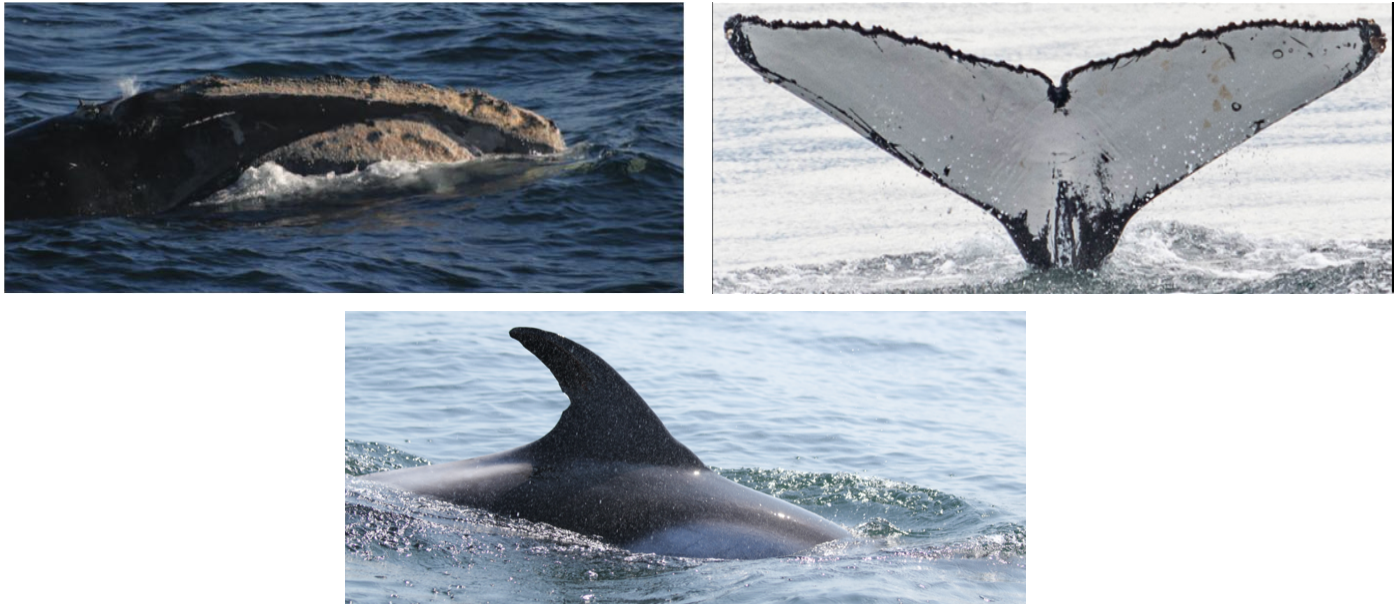
\includegraphics[scale=0.6]{Chapter2/figs/body-part-examples.png}
	\end{center}
	\caption[Examples of the main body parts utilised in cetacean photo-id.]{Examples of the main body parts utilised in cetacean photo-id. Left: callosities present on the head of a northern right whale (\textit{Eubalaena glacialis}) \cite{perrin_encyclopedia_2009}. Right: fluke of a humpback whale (\textit{Megaptera novaeangliae}) \cite{cheeseman_happywhale_2019}. Bottom: dorsal fin of a common bottlenose dolphin (\textit{Tursiops truncatus}) \cite{trotter_ndd20_2020}.
	}
	\label{fig:body-parts}
\end{figure}

During photo-id surveys, researchers will often focus on long lasting markers such as body-part shape, nicks, notches, and pigmentation which have been shown to be stable throughout the life of the animal \cite{wursig_photographic_1977, lockyer_observations_1990, mann_cetacean_2000}. In some cases, secondary markers, those which may heal and are thus not stable such as scarring, may also be utilised for identification. Markers may be anthropogenically caused, for example from collision with a vessel, or natural, for example from encounters with prey. Examples of prominent markings used in dolphin photo-identification surveys can be seen in Figure \ref{fig:nicks-scarring-scratching-pigmentation}.

\begin{figure}
	\begin{center}
		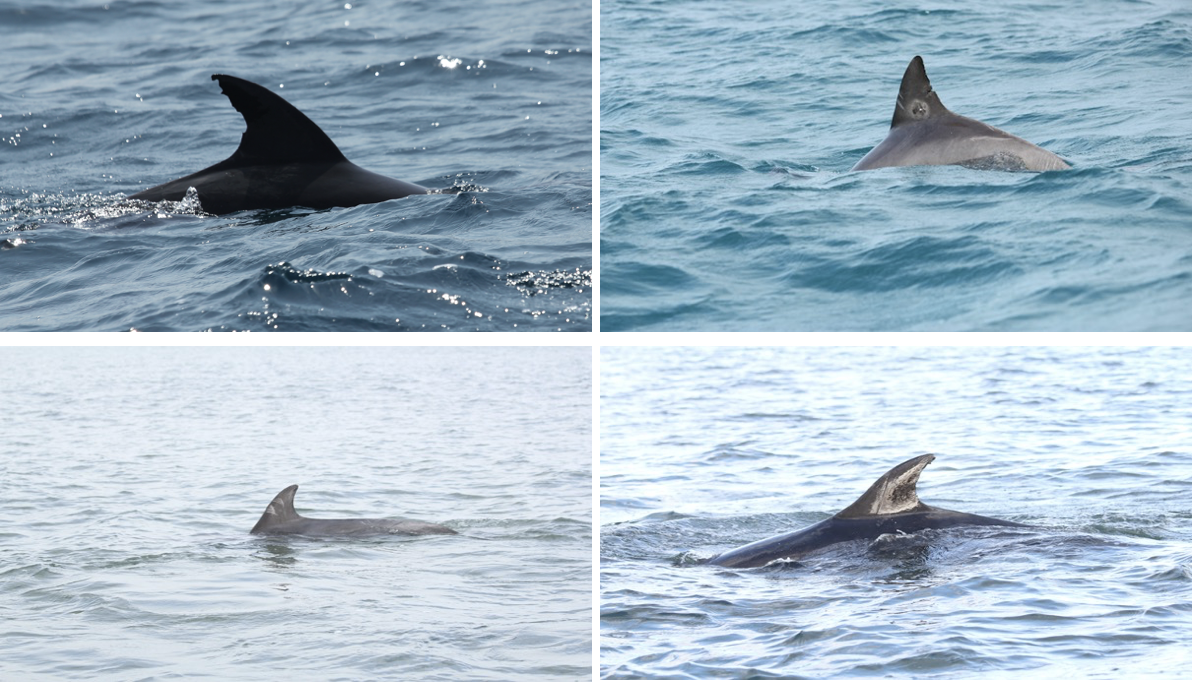
\includegraphics[scale=0.6]{Chapter2/figs/nicks-scarring-scratching-pigmentation.png}
	\end{center}
	\caption[Examples of prominent markings used during dolphin photo-identification surveys.]{Examples of prominent markings used during dolphin photo-identification surveys. Top Left: nicks. Top Right: scarring. Bottom Left: scratches. Bottom Right: pigmentation.
	}
	\label{fig:nicks-scarring-scratching-pigmentation}
\end{figure}

Scarring is of particular use when identifying Risso's dolphins, a species well known for the persistent nature of their scars caused by tooth rakes from other Risso's \cite{mariani_analysis_2016}. The use of pigmentation for photo-id is also present in the literature for species such as striped dolphins (\textit{Stenella coeruleoalba}) where it can be considered a primary marker \cite{rosso_colour_2008}.

Regardless of the species being analysed or the body-parts used during photo-id it is imperative that the process is standardised, allowing for work to be compared over spatial and temporal scales. This process began in 1988 through workshops held by the International Whaling Commission \cite{hammond_individual_1990}, with further recommendations published in 2015 by Urian \textit{et al.} \cite{urian_recommendations_2015}.

This standardisation process requires some assumptions to be universally made. For one, all of the markers must be considered stable, that is, they must not fade over the years. Even if a photo-id study only occurs over a few years, the markers utilised must be stable enough so that if another survey is conducted in the same area in later years, individuals from the first study must still be identifiable -- providing useful information to health assessments, population estimates, and residency surveys. This stability reduces false positives, where one individual is recorded as multiple over time. Second, the markers must be considered individually unique. Those chosen to identify an individual must not overlap with other individuals in the survey area. This reduces the chance of false negatives, where multiple individuals are recorded as one. Chosen markers must also allow for a consistent re-sighting probability over time. This is critical for abundance estimates, ensuring that an individual's chosen markers provide it with the same chance of being spotted in one year as another. As such, it is extremely important that photo-id methodologies are standardised, both at an international level and between researchers in the same organisations. For a full review of marine photo-id methodologies, efforts to date, and the assumptions made during data collection, see Hammond \textit{et al.} \cite{hammond_estimating_2021}.

Because of the assumptions which must be adhered to, as well as the manual nature of photo-id, there are many downsides to the process. Being able to identify individuals relies on high quality photographs. Thanks to the advent of digital photography and the relative inexpensiveness of cameras capable of capturing large megapixel images, this is less of an issue than before, although it must still be considered. Surveys can also only be undertaken in good weather conditions in terms of sea state and lighting, both of which can affect the chance of an accurate match. These conditions are harder to meet in some areas of the world, reducing the suitability of photo-id for some geographic areas. Conditions, as well as the nature of the animal itself, may make photographing both sides of the individual impossible. Markings are rarely duplicated on both sides of an individual, and thus not having both sides may make matching difficult. For example, an individual may have an extremely distinctive marking on the left side of their dorsal fin, however if only the right side of the individual has been captured, when the left side is also eventually photographed it may be labelled as a new individual as no previous examples of the individual's left side exist in the catalogue. If the individual has a very distinct fin shape then this issue can be overcome, although this may not always be possible. As such, individuals may not be added to a catalogue without both sides of the fin available for later comparison. 

Furthermore, photo-id as a whole is extremely labour intensive. Unlike land-based camera trap systems, marine-based photo-id surveys require a large human effort. Staff are needed not just for photographic purposes, but also for piloting of vessels. As the surveyed animals are free roaming, large spatial areas must be covered, and there is no guarantee of encountering them during a given day. Back on land, the captured photographs must then be manually analysed and the individuals in them identified. This can often take longer than the entire data collection period. Due to the labour intensiveness of the photo-id process, it can also be extremely costly to undertake. Staff need to be paid, vehicles need to be fuelled, and equipment must be maintained. Because of this, any solutions which may speed up the photo-id process, provided they are robust, would be welcomed both by researchers and their funding bodies. 

\section{Machine Learning: Supervised vs Unsupervised Approaches}\label{ch:Background,sec:DLIntro,sub:supervisedVsUnsupervisedLearning}

Before it is possible to understand how deep learning and computer vision can be utilised to aid in the photo-id process, it is important to discuss the differences between supervised and unsupervised machine learning.

\textbf{Supervised learning} tasks are those where the model can be trained using an input and expected output value pair, known as a ground truth. This technique lends itself well to tasks such as classification, where an input can be mapped to a set of defined output classes, or in regression where an input can be mapped to a continuous output space. 

Training is performed by splitting the available data into training and test sets, with the former being used to train the model and the latter being used to test the model's performance on previously unseen data. Both the training and test set contain ground truth data, but only the training set's influences the generalisation of the model. For example, in the case of a dog verses cat classifier a dataset may contain one thousand images, some labelled as \texttt{dog} and some as \texttt{cat} (the ground truths). This data will then be split randomly into a training and a test set; for example 80\% of the data used for training with 20\% used for testing. The classifier will then iterate through the training set, using the ground truth values to train the network's parameters in a way to best generalise the model. After training has been completed the model will then be evaluated against the test set. Each data point will be processed by the model and a prediction outputted, which is then compared to the unseen ground truth to provide an evaluation of the model's performance.

\textbf{Unsupervised learning} tasks are, in contrast, those where prior ground truths for the data are not available. This approach lends itself well to clustering and aiding in the understanding of the underlying data structure. These unsupervised algorithms, such as K-Means clustering \cite{hartigan_algorithm_1979}, are not provided human guidance on how to group the data given, but are rather left to discover interesting structure patterns on their own. 

Taking the \texttt{dog} and \texttt{cat} labelled data again as an example, this data could be clustered in an unsupervised manner. Asking the clustering algorithm to provide two clusters for the data  (e.g. $K = 2$), a model could be trained to split the data with all dogs in one cluster and all cats in the other, without having to be told which images are dogs and which are cats. However, due to the unsupervised nature of the learning process, the model is equally as likely to cluster the data based on whether the animal is, for example, sitting or standing. 

\section{A Brief Introduction to Deep Learning}\label{ch:Background,sec:DLIntro}

Deep learning, a subfield of machine learning, aims to create artificial networks to complete tasks through a learning process. These computational models are made up of neurons and are often multiple layers deep. Earlier layers represent basic abstractions building up from this as you go deeper into the network. Layers at the deepest points can, based on information passed to them from higher layers, begin to provide estimations of answers to a given problem. The ability to learn directly from the data provided is the key difference between deep learning and more classical machine learning techniques, which often require considerable domain expertise to design a feature extractor allowing for raw data values, such as pixels, to be transformed into a feature vector suitable for a model to learn.

Deep learning models in contrast are capable of learning to perform tasks such as classification on raw data values through multiple layers of simple non-linear transformations. For example in the case of computer vision, earlier layers of neurons are optimised by the network itself to learn lines and basic shapes, middle layers may be optimised to learn more complex ideas such as how these lines and shapes fit together, with the final layers providing an output of object label (e.g. \texttt{dolphin}). It should be stressed however that the features these layers are looking for are not specified by humans, but rather learned from the data by updating their parameters predominantly through optimisations such as stochastic gradient descent (see Section \ref{ch:Background,sec:DLIntro,sub:stochasticgradientdescent} for further details).

This ambition to create artificial networks similar to how the brain operates stems mainly from work undertaken in 1943 by McCulloch and Pitts \cite{mcculloch_logical_1943} in an attempt to understand how neurons in the brain allow for the understanding of complex patterns. This model formed the basis of future work into machine learning, and thus deep learning. This work continued at small scale for many years. It has only been recently, thanks to advances in availability of large scale datasets needed to train these networks and power of the computing resources available, that deep learning research has accelerated. The transition to training on clusters of high-powered Graphical Processing Units (GPUs)\nomenclature[z-GPU]{GPU}{Graphical Processing Unit} has allowed for a significant speed-up in both model training and inference time compared to traditional Central Processing Units (CPUs)\nomenclature[z-CPU]{CPU}{Central Processing Unit}, allowing for a higher amount of prototyping in a smaller time frame \cite{luo_artificial_2005}. Further to this, the advent of cloud computing has allowed for much more cost-effective model development. 

Development of deep learning models has been helped greatly through the creation of standard programming frameworks. Google's Tensorflow \cite{abadi_tensorflow:_2016} and Meta's PyTorch \cite{paszke_automatic_2017} allow researchers to develop models faster than before due to their reduction in the amount of boiler-plate code needed, with these frameworks often doing a lot of the heavy lifting in the background. Further advances have been made through the availability of large scale coarse-grained datasets such as MNIST \cite{lecun_gradient-based_1998} and ImageNet \cite{deng_imagenet:_2009}, allowing for common baselines to be adopted by the computer vision community and for the introduction of transfer learning, allowing for the reuse of models trained on one task to be utilised for another \cite{pan_survey_2010}. Furthermore, additional regularisation techniques have provided improvements to model accuracy. Notable examples of this in the literature which are now commonplace in deep learning models include dropout \cite{srivastava_dropout:_2014}, batch normalisation \cite{ioffe_batch_2015}, and stochastic gradient descent with warm restarts \cite{loshchilov_sgdr:_2016}. The use of data augmentation is also commonplace. This is where existing data is perturbed randomly to create new, artificial data. Examples of image data augmentation include simple perturbations such as random horizontal and vertical flipping, and cropping, as well as more complicated techniques like Gaussian blurring, perspective shifting, and colour jitter.

\subsection{Optimising Deep Learning Networks}\label{ch:Background,sec:DLIntro,sub:stochasticgradientdescent}

In order to generalise deep learning models, there exists a need to optimise the parameters within each individual neuron. These parameters can either be weights that control the strength of the connection between two neurons, or biases -- some constant additional input. Most commonly, this is performed using gradient descent to minimise some loss function (a measure of distance between ground truth and model prediction) with respect to a dataset. If this function were to be visualised on a graph each parameter would be represented by an axes, resulting in a hyper-surface with millions of dimensions in the case of deep learning models. The goal of network optimisation is to find the minimum point on the hyper-surface, as this would give the parameter values which produce the smallest loss. 

This hyper-surface is non-convex however, which can result in multiple local minimums. In order to find the (hopefully global) minimum point on the hyper-surface, during training the model's weights must be updated iteratively in the opposite direction of the gradient of the loss function's hyper-surface. As such, this follows the direction of the slope of the hyper-surface downhill until a minima, an area where the loss is lowest, is reached \cite{ruder_overview_2016}. 

Before the advent of deep learning and big data, it was common for the whole training set to be used to compute the gradient at each iteration; however due to the size of modern day datasets this is no longer possible due to the computational cost this would impose on the system. As such, batches, a small random subset of the larger dataset, are often used to give an estimation of the overall loss gradient.

In order to achieve this, a process known as mini-batch stochastic gradient descent (SGD)\nomenclature[z-SGD]{SGD}{Stochastic Gradient Descent} is commonly used. At each iteration of SGD, a mini-batch which contains some subset of the dataset is utilised rather than the entirety. The loss for this batch is calculated and used to step down the gradient slope, rather than the sum of the loss' gradient over all training examples. As only some subset of the data is taken per iteration, the path down the slope of the minima is far noisier and more random than the path obtained when using all examples. Whilst this results in a longer convergence time to the minima compared to non-batch gradient descent, this is outweighed by the fact that the entire dataset does not need to be loaded into memory at once, allowing for computation to be performed using machines which are, relatively speaking, more resource constrained. The use of SGD often quickly leads to a good set of model weights compared to other, more elaborate techniques \cite{bottou_tradeoffs_2008}. 

In recent years there have been efforts to modify SGD in an attempt to improve model optimisation. The most commonly seen optimisers within production code include SGD with warm restarts (SGDR)\nomenclature[z-SGDR]{SGDR}{Stochastic Gradient Descent with Restarts} \cite{loshchilov_sgdr:_2016}, Momentum \cite{qian_momentum_1999}, RMSProp \cite{tieleman_lecture_2012}, Adam \cite{kingma_adam:_2014}, and AMSGrad \cite{reddi_convergence_2019}. Work in this thesis utilises SGDR and Adam primarily -- for a more in-depth discussion of these, see Section \ref{ch:cetDet,sec:ModelSelection,sub:TrainingHyperparameters,subsub:learningRateOptimisers}. All of these optimisers attempt to stop the problem of getting stuck in local minima rather than the global minimum of the overall loss function (although it should be noted that it is very unlikely the global minimum will ever be reached during the training process). However, recent studies show that the problem of local minima is not as big as first thought and, regardless of initial conditions, vanilla SGD rarely gets stuck in local minima \cite{dauphin_identifying_2014, choromanska_loss_2015}.

\subsection{Backpropagation}\label{ch:Background,sec:DLIntro,sub:backprop}

As discussed in Section \ref{ch:Background,sec:DLIntro,sub:stochasticgradientdescent}, the weights and biases in each neuron can be learnt and optimised using optimisers such as SGD. However, it is also important to understand how a weight's or bias' effect on the gradient is computed. This can be performed relatively quickly using backpropagation, or the backward propagation of errors algorithm. Before delving too deep into deep learning, it is of imperative importance to understand backpropagation; it is after all often cited as one of the cornerstones of deep learning \cite{alber_backprop_2018}.

Backpropagation was originally described in Linnainmaa's Masters thesis from 1970 \cite{linnainmaa_representation_1970}, although its effect was not fully realised until 1986, when Rumelhart \textit{et al.} discussed the advantages to using backpropagation over other learning approaches \cite{rumelhart_learning_1985}. In recent years multiple works have provided updates and improvements to the original backpropagation algorithm, however none have seen wide-scale adoption \cite{bengio_use_1994, lillicrap_random_2014, lee_difference_2015, nokland_direct_2016, liao_how_2016}. 

During each training step, the output for each example input is predicted using the weights and biases of each node in the network. Any error in the output prediction can be represented as a weighted sum of the error in the node's weights and biases. As such, this error can be corrected by changing these weights and biases on a per node basis. However, as nodes between layers can be connected together and influence each other (network architecture depending), it can be computationally expensive to determine the change required for each node in isolation.

The backpropagation algorithm provides a computationally efficient way of calculating the change required with respect to the gradient of the loss function. Operating on a per node basis, the algorithm works backwards through the network determining how each node's weights and biases should be updated. For each node, the calculated gradients of the loss function are passed backwards through the network to the preceding directly connected nodes to be used in their calculations, up until the input layer. As such, the standard backpropagation algorithm is, in essence, the chain rule (a formula for computing the derivative of compound functions), and provides a far more computationally efficient way of calculating the overall gradient loss compared to calculating each layer's gradient loss in isolation. Further efficiencies have been made thanks to deep learning frameworks implementing backpropagation in a way that takes advantage of GPUs, leading to extremely efficient computations when performing deep learning tasks.

\section{Deep Learning for Computer Vision}\label{ch:Background,sec:DLforCV}

The field of computer vision, allowing computers to gain and interpret knowledge from image and video data, is one area where deep learning has excelled \cite{voulodimos_deep_2018}. Generalisable concepts such as Convolutional Neural Networks (CNNs)\nomenclature[z-CNN]{CNN}{Convolutional Neural Network} have quickly become commonplace for solving computer vision tasks, in most cases replacing the need for hand-crafted pipelines specialised to the task at hand, thanks to their ability to learn complex patterns in data where there is a strong spatial and temporal dependency between the values. This ability is essential for processing image data which is, at its most basic level, a tensor of pixel values. These tensors are three dimensional, representing an image's height, width, and depth, where depth is dependant on the colour model used to represent the image. The most common of these models is RGB which has channels representing the red, green, and blue colours present in an image; a matrix representing an RGB image will have a depth of three. Other colour models have varying depth values, a greyscale image would have a depth of one for example, whilst a CMYK image which has cyan, magenta, yellow, and black colour channels would have a depth of four. As can be imagined, these matrices can very quickly reach unworkable sizes. An RGB image at 1080p resolution for example would require a tensor of size 1920x1080x3, or 6,220,800 values. Thankfully, CNNs utilise a set of standard operations which are capable of reducing image sizes down to a more workable form whilst still retaining key features which allow for inference to occur. 

\subsection{Convolutional Neural Networks}\label{ch:Background,sec:CNN,sub:CNN}
Modern CNNs are composed mostly of three main layer types; convolutional layers, pooling layers, and fully connected layers. Each of these layers will perform some operation on the input matrix passed to it, and provide a transformed output to the subsequent layer(s). These layers can be stacked in various orientations to build different CNN architectures.

\subsubsection{Convolutional Layers}\label{ch:Background,sec:CNN,sub:CNN,subsub:convolution}

The convolutional layer is the workhorse of the CNN, performing the vast majority of the operations required. Convolutional layers utilise what is known as a kernel in order to efficiently extract features from an input image matrix. A kernel is a matrix, most commonly 3x3 or 5x5 in size, which represents some weighting refined through training. This kernel is slid over the input data computing the dot product between the weights and the section of the input matrix it is currently over, before summing these into a single value and passing them through an activation function. This gives an output matrix of features represented by the weighted sum of the input, known as a feature map. These feature maps generally represent basic shapes at shallow levels, which are then built on as the model gets deeper \cite{kim_convolutional_2017}. The kernel process can be performed multiple times over the same input using different weightings, giving multiple output feature maps. A visual representation of a convolutional layer can be seen in Figure \ref{fig:convolution}.

\begin{figure}
	\begin{center}
		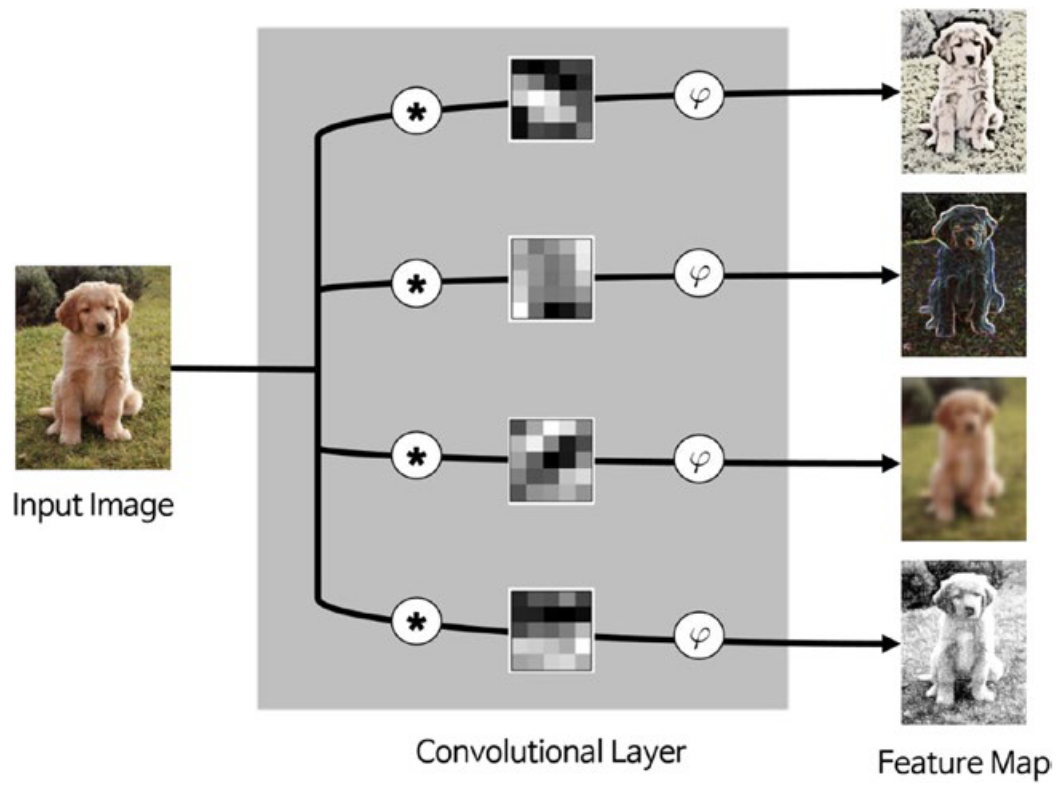
\includegraphics[width=0.6\linewidth]{Chapter2/figs/convolution.png}
	\end{center}
	\caption[A visual representation of convolution.]{A visual representation of convolution. An image, left, is fed into a convolutional layer. The input is passed through a convolution operation, $*$. The greyscale blocks in the centre of the convolutional layer represent the kernels passed over the image. $\varphi$ represents the activation function the kernel output is fed to. This process results in multiple outputted feature maps. Image from \cite{kim_convolutional_2017}.}
	\label{fig:convolution}
\end{figure}

In the case where there are multiple input dimensions (such as an RGB image), kernels are required to operate over all dimensions. As such, the resulting feature maps are summed element-wise, along with some bias term, to produce a single output map. The size of the kernel determines the number of input features which are combined to give the new output feature map, although the size of the resulting map is determined also by two other properties; stride and padding. Stride refers to the distance in pixels the kernel will move when performing the next input mapping. For example, a stride of 1 would result in the kernel sliding along one pixel value each time, resulting in an output feature map of equal size to the input, whereas a stride of 2 would skip every other pixel, reducing the output feature map by half. Figure \ref{fig:kernels} shows a visualisation of the kernel process with a stride of 2.

A problem can arise during convolution when the kernel reaches the edges of the input matrix. As there is nothing past the edge values, these must be trimmed as they can never be in the centre of the kernel. This is known as `valid' padding, and can cause a reduction in the size of the matrix which may be detrimental when an output feature map of equal or greater size than that of the input is required. To avoid this, `same' or zero padding can be utilised whereby zeros are added to the edges of the matrix, allowing the input and output feature maps to be of the same size. `Full' padding can also be utilised, whereby multiple rows and columns of zeros are added such that all non-padding values are visited equal amounts of times by the kernel. This has the effect of increasing the size of the output feature map.

\begin{figure}
	\begin{center}
		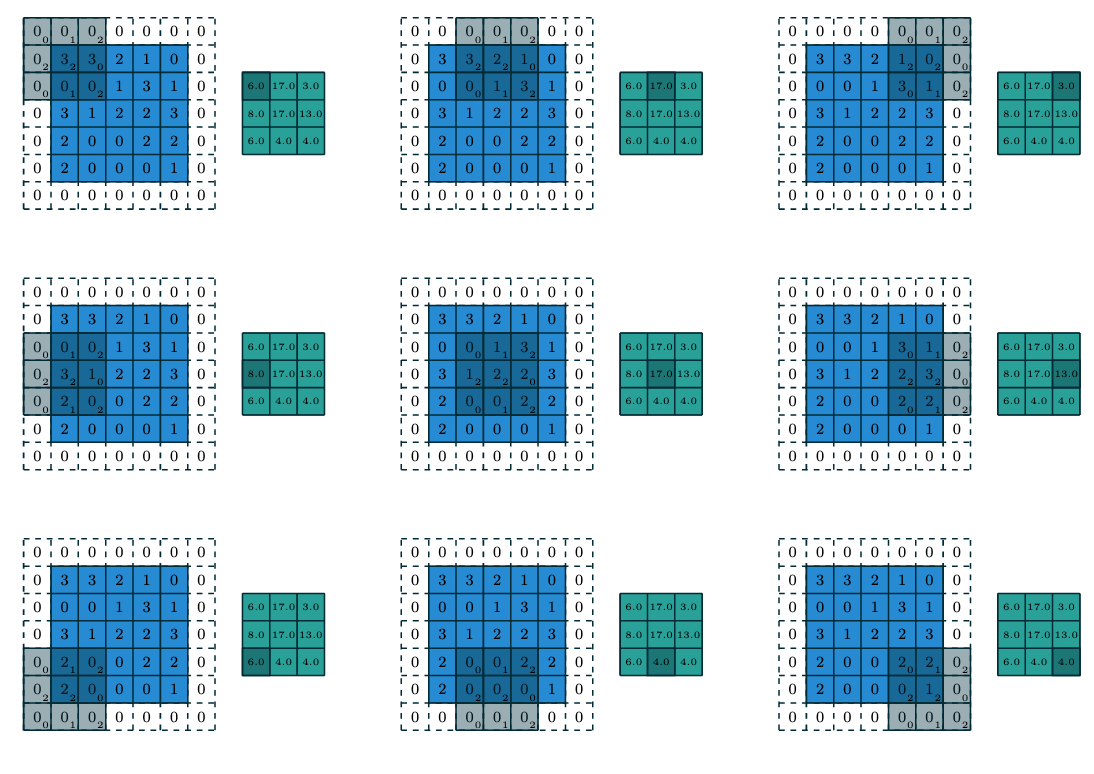
\includegraphics[width=\linewidth]{Chapter2/figs/kernel.png}
	\end{center}
	\caption[A kernel, represented by the grey squares, operates over a padded input matrix, blue, with a stride of 2 to produce an output feature map, green.]{A kernel, represented by the grey squares, operates over a padded input matrix, blue, with a stride of 2 to produce an output feature map, green. Note that the kernel's weights are denoted by the number in the lower right of each box and the input pixel value is denoted by the number in the middle of each box. Image from \cite{dumoulin_guide_2018}.}
	\label{fig:kernels}
\end{figure}


\subsubsection{Pooling Layers}\label{ch:Background,sec:CNN,sub:CNN,subsubsec:pooling}

Pooling layers help reduce the computational complexity of the convolutions performed by the CNN. This is achieved by reducing the spatial dimensions of the input ready for the next convolutional layer through the use of some function applied over batches of the input pixel values, similar to how a kernel operates in a convolution layer by sliding over the image. Pooling only affects the width and height of the input, not the depth, as all depth channels are required to keep the colour mapping of the image intact. 

Pooling as such inevitably leads to a reduction in the amount of information available to subsequent layers; this is advantageous however as it leads to less computational complexity, aiding in the minimisation of overfitting in the model. 

A number of different pooling layer architectures exist in the literature, such as max pooling which only keeps the maximum pixel value in the batch, average pooling \cite{boureau_theoretical_2010} which outputs the mean of all pixel values in the batch, and stochastic pooling \cite{zeiler_stochastic_2013} which selects an output pixel value from each batch based on a probability distribution. For a review of current pooling methods, see Gholamalinezhad \textit{et al.} \cite{gholamalinezhad_pooling_2020}.

\subsubsection{Fully Connected Layers}\label{ch:Background,sec:CNN,sub:CNN,subsubsec:fullyConnected}

Fully connected layers take feature maps produced by the preceding convolutional and pooling layers and reduce these down to a single $N$-dimensional vector. In the case of the last layer of a network geared towards a classification problem, $N$ represents the total number of possible classes the network was trained to identify, with the values in the vector representing the input's class probabilities.

An activation function is responsible for deciding which neuron in the layer passes its value to the layer below by computing the weighted sum of the inputs and passing the result through some non-linear function. This has the effect of scaling the layer's output to within some defined limits. Multiple common activation functions exist in the literature, such as the tanh function which scales values to between -1 and 1. The use of the softmax activation function is commonly used in the last layer of a classification network in order to determine the class probabilities mentioned previously. Softmax takes the exponents of each input and normalises them by the sum of all inputs, giving values between 0 and 1. Outputted $N$-dimensional vectors can then be considered a feature map in their own right for further processing \cite{krizhevsky_imagenet_2012} or as a category for classification as the last layer of the network \cite{girshick_rich_2014}.

\begin{figure}[!hb]
	\begin{center}
		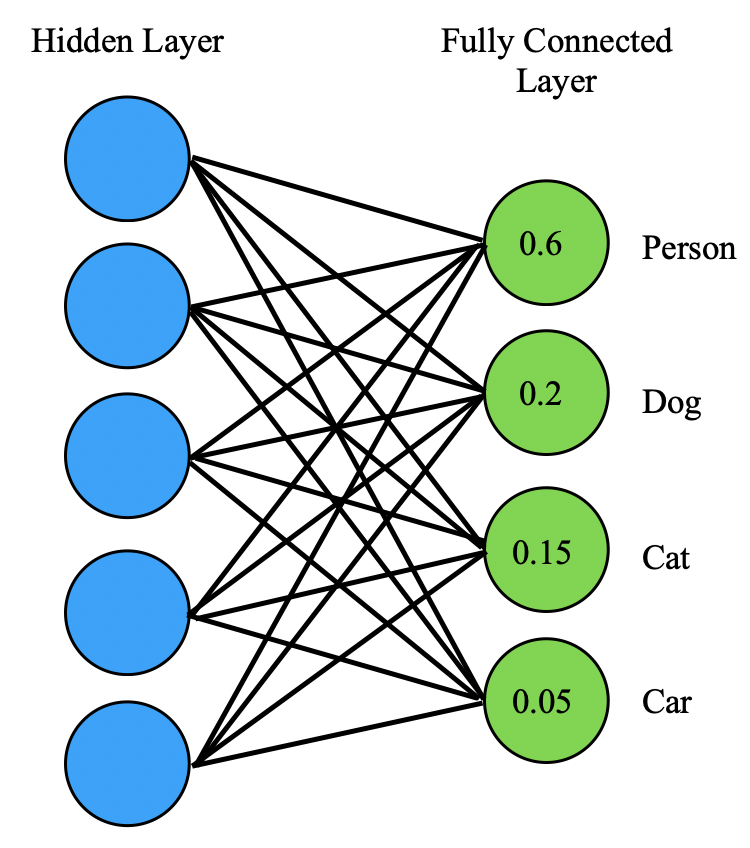
\includegraphics[scale=0.45]{Chapter2/figs/fully-connected.png}
	\end{center}
	\caption[A visual representation of the final stages of a classification network.]{A visual representation of the final stages of a classification network. The blue circles represent the final hidden layer in the network, with the green circles representing the fully connected layer. Each neuron in the hidden layer is connected to all neurons in the fully connected layer. The value in the hidden layer's neurons represents the activations after softmaxing, with the label denoting the class represented by the neuron. The network has predicted the input to be of class \texttt{Person}. Note that additional CNN layers would be present before the hidden layer.}
	\label{fig:fully-connected}
\end{figure}

Figure \ref{fig:fully-connected} shows the final layers of a network whose aim is to classify an image into one of four classes. At the end of this network is a fully connected layer which takes a feature map from the preceding hidden layer, and produces as output four values between 0 and 1. Each of these values is required to be outputted by its own neuron, resulting in a fully connected layer with four neurons where each neuron represents a possible class for the input image. The image's classification is provided by whichever neuron outputs the highest value. 

\subsubsection{Layer Architectures}\label{ch:Background,sec:CNN,sub:CNN,subsub:layerArchitecture}

Using the three layer types described previously it is possible to create an infinite number of CNN architectures. There is no guarantee that every possible architecture will perform well however (indeed, one possible combination would be a single fully connected layer, which would not perform well at all). Whilst it may be advantageous for certain areas of research to create their own custom CNN architecture, either through trial and error or the more recent approach of Neural Architecture Search \cite{elsken_neural_2018}, due to the computational expense of identifying good networks many choose not to perform this work. For the vast majority of cases, there exists in the literature well-defined generalised CNN architectures which have demonstrated that they produce good results, and it is often these architectures which are utilised for computer vision tasks. 

LeNet \cite{lecun_gradient-based_1998} was the first well defined CNN architecture. LeNet was only seven layers deep, but performed well enough to be applied by some banks for automatic recognition of numbers on cheques. It was not until around 2012 that more attention was paid to these defined architectures however, thanks to AlexNet \cite{krizhevsky_imagenet_2012}. Utilising a similar but deeper architecture to LeNet, with more filters and a larger number of stacked convolutional layers, AlexNet also included now commonplace deep learning building blocks such as dropout, whereby nodes in the model are intentionally not updated during a training step with some probability to aid model generalisability \cite{srivastava_dropout:_2014}, max pooling \cite{boureau_theoretical_2010}, and Rectified Linear Unit (ReLU)\nomenclature[z-ReLU]{ReLU}{Rectified Linear Unit} activation functions; the most popular non-linear activation function currently in deep learning, especially in computer vision \cite{he_delving_2015}.

 In 2014, Google introduced GoogleNet, also known as an Inception architecture, to the ILSVRC14 competition \cite{szegedy_going_2015}. This architecture achieved a top-5 error rate of 6.67\%, very close to what untrained humans could achieve on the competition dataset, ImageNet \cite{krizhevsky_imagenet_2012}. This was achieved through a 22 layer deep CNN utilising several small convolutions, reducing the number of parameters from 60 million in AlexNet to 4 million in GoogleNet. 

Finally ResNet \cite{he_deep_2015} was introduced a year later at ILSVRC15. This architecture can be up to 152 layers deep, and achieved a human-beating top-5 error rate of 3.57\%. Shallower versions of ResNet exist, such as ResNet50 and ResNet101, which are 50 and 101 layers deep respectively.

\subsection{Object Detection}\label{ch:Background,sec:objectDetection}

Thanks to advancements in deep learning technology and the creation of standardised architectures, CNNs are now utilised en masse to perform tasks such as object detection, attempting to identify distinct regions containing task-specific classified objects in images and video. Whilst this is often performed in one of two ways, it is important to note that all object detection is still in essence a series of tasks performed via network layers. 

\subsubsection{Region Proposal Networks}\label{ch:Background,sec:objectDetection,sub:RPN}

The first, known as a Region Proposal Network (RPN)\nomenclature[z-RPN]{RPN}{Region Proposal Network}, attempts to find image regions likely to contain objects of given classes. Training data is usually provided in the form of bounding boxes drawn around objects of interest and labelled with the corresponding class. One of the most common and widely used RPN architectures is derived from the R-CNN, or Regions with CNN features, architecture \cite{girshick_rich_2014}. R-CNN utilises a selection search \cite{uijlings_selective_2013} to generate 2000 Regions of Interest (RoIs) representing the most likely areas of the input image to contain a class example. By limiting the number of RoIs generated this allows for fast computation compared to operating on every possible region in the image. The proposed RoIs are then fed through a CNN to be classified. See Figure \ref{fig:r-cnn} for a visual representation of the R-CNN pipeline. Example proposed RoIs can be seen in Figure \ref{fig:rpn-randoms}.

\begin{figure}
	\begin{center}
		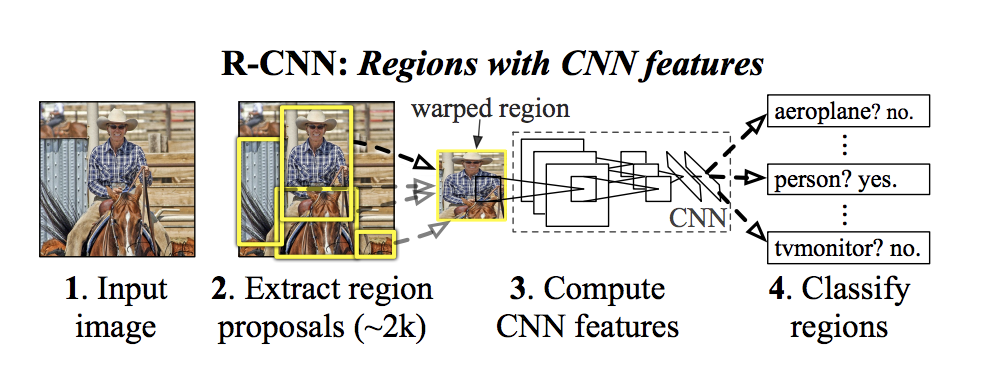
\includegraphics[scale=0.45]{Chapter2/figs/r-cnn.png}
	\end{center}
	\caption[The R-CNN pipeline.]{The R-CNN pipeline. (1) Input images are passed to (2) a region proposal network, extracting around 2000 RoIs. (3) Each RoI is then resized and passed through some CNN backbone architecture. (4) The output of the CNN corresponds to the RoI's classification and confidence score. Any RoIs with confidences above some defined threshold are outputted by the model. Image from \cite{girshick_rich_2014}.}
	\label{fig:r-cnn}
\end{figure}

\begin{figure}
	\begin{center}
		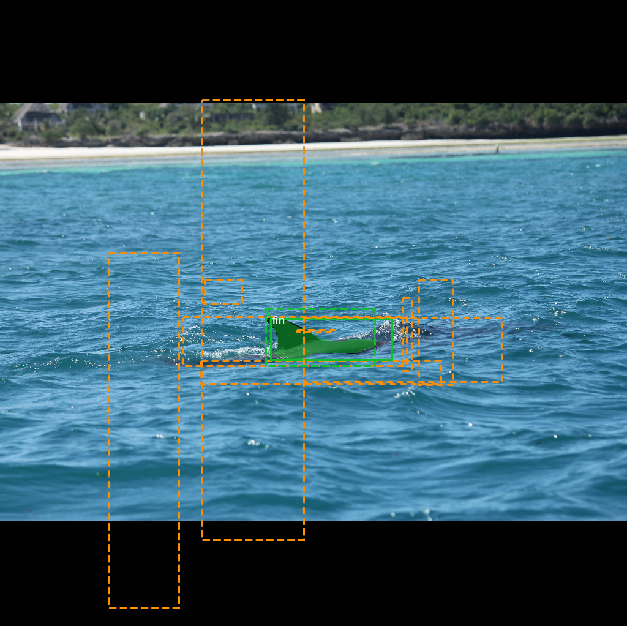
\includegraphics[scale=0.3]{Chapter2/figs/rpn-ten-random-orange.png}
	\end{center}
	\caption{An example of RoIs generated on an image by an RPN, showing 10 random proposals.}
	\label{fig:rpn-randoms}
\end{figure}

Utilising selection search leads to a high recall rate thanks to the large amount of proposals, as there is a high probability that some of these proposals will contain RoIs with objects being searched for. However, this can be time consuming and computationally expensive (although less computationally expensive than just sliding a window over the full image) as the network needs to classify the 2000 region proposals generated. Detection can also be slow using an R-CNN and, with the selection search being fixed, no adaptive learning takes place here which may lead to bad region proposal generation. 

Some of these time drawbacks were fixed in a later version of R-CNN, known as Fast R-CNN \cite{girshick_fast_2015}. Rather than feeding the region proposals generated to the CNN, this algorithm instead feeds the input image to the CNN and generates a feature map. RoIs can then be taken from the feature map using selection search and warped into a shape suitable for the pooling layer, before being reshaped again into a fixed size for the fully connected layer. This is advantageous as it allows for the reuse of some computations and for backpropagation to occur throughout the network, greatly improving run times. This also means however that the runtime is determined by how fast RoIs can be generated. 

To fix this issue, Faster R-CNN was developed \cite{ren_faster_2015}. Now instead of utilising selection search to generate the RoIs, a separate network can be utilised to predict RoIs which are then used to classify images within the regions. As such, training now occurs with four losses: 

\begin{enumerate*}
	\item An object/not object classification from the RPN;
	\item The RoI shift;
	\item The object classification;
	\item Final bounding box co-ordinates.
\end{enumerate*}

Building upon Faster R-CNN, Cascade R-CNN \cite{cai_cascade_2018} aims to reduce the overfitting during training and quality issues at inference through the use of a proposal sub-network to produce preliminary detection hypotheses which are then processed by an RoI sub-network. 

\subsubsection{Detection Without Proposals}\label{ch:Background,sec:objectDetection,sub:noProposals}

One issue with all RPNs is that they generally take a significant amount of time in order to classify objects in images, with the bottleneck being the region proposal generation. Because of this, there are algorithms which attempt to remove the region proposals altogether and instead look at the whole image. The input image is divided into an equal size grid. Within each square of the grid a set number of bounding boxes are generated, which the CNN provides classification confidences for. Any above a set threshold are used to locate the object within the image. These algorithms are essentially one large CNN rather than splitting into a CNN and an RPN and are thus much faster although are not as accurate, especially on smaller objects due to the spatial constraints of the algorithm. Examples of detection without proposal systems include YOLO \cite{redmon_you_2016} (including the more recent state-of-the-art versions \cite{bochkovskiy_yolov4_2020, li_yolov6_2022, ge_yolox_2021, li_yolov6_2023, xu_pp-yoloe_2022}), SSD \cite{liu_ssd:_2016}, DINO \cite{zhang_dino_2022}, RetinaNet \cite{royo-miquel_retinanet_2021}, and EfficientDet \cite{tan_efficientdet_2020}. 

\subsection{Semantic Segmentation}\label{ch:Background,sec:semanticSegmentation}

Along with object detection, semantic segmentation is one of the key research areas in computer vision. Rather than provide RoI bounding boxes as output, semantic segmenters instead output a class label for each pixel in the image. A group of connected pixels of the same class is known as a mask. An example semantic segmentation mask can be seen in Figure \ref{fig:semantic-eg}.


\begin{figure}
	\begin{center}
		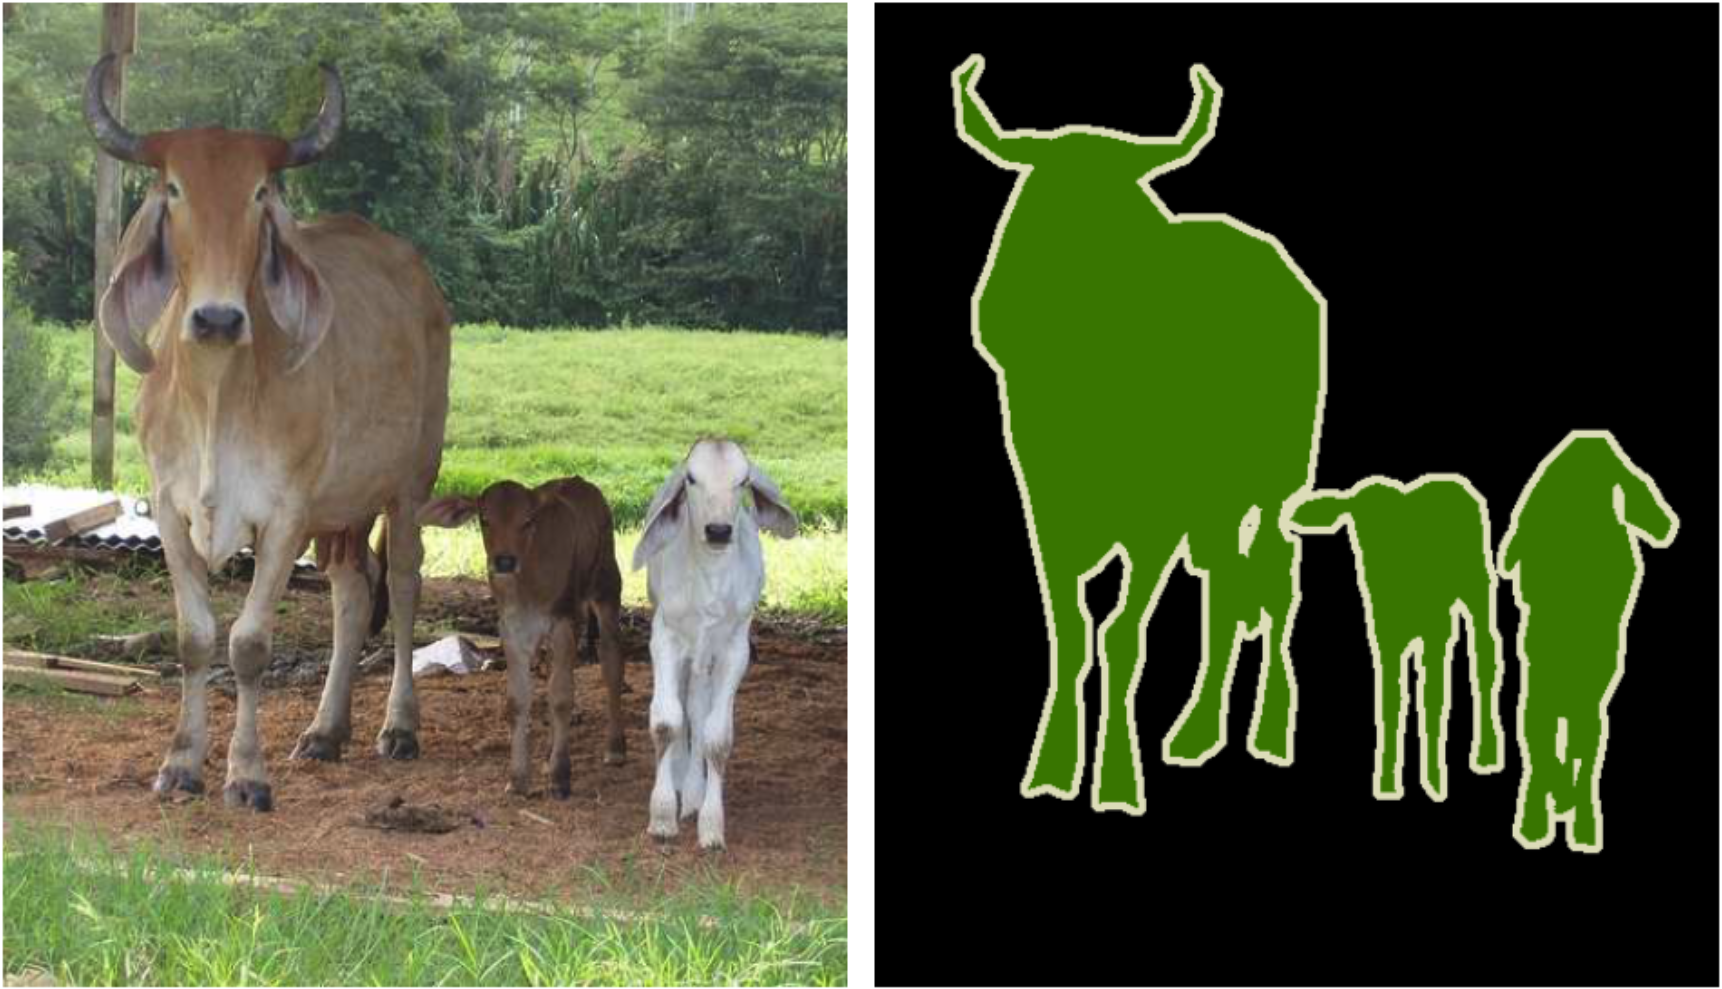
\includegraphics[scale=0.15]{Chapter2/figs/semantic_segmentation_updated.png}
	\end{center}
	\caption[Left: an example input image to a semantic segmentation model. Right: the resultant semantic segmentation mask for the given input image.]{Left: an example input image to a semantic segmentation model. Right: the resultant semantic segmentation mask for the given input image. All pixels which make up any \texttt{cow} object have been classified as one \texttt{cow} mask. Image from \cite{noh_learning_2015}.}
	\label{fig:semantic-eg}
\end{figure}

In general, semantic segmenters can be thought of as having two main components; an encoder, usually a pre-trained classifier built with a standard detection architecture such as ResNet \cite{he_deep_2015}, and a decoder whose job is to project the coarse-grained features learnt by the encoder to a fine-grained pixel space. There are two main ways to approach this decoding step.

The first is to use an RPN to perform region based semantic segmentation, extracting the regions from an image and then describing them. Each pixel of the image is then given a classification based on which highest scoring region it is contained in. Note that any pixels not in a region are given the class label of \texttt{background}. This is achieved through the use of a lightweight binary classifier operating over multiple proposal boxes, known as anchors, covering the image at different scales. Each anchor is given an object score denoted by Intersection Over Union (IOU)\nomenclature[z-IOU]{IOU}{Intersection Over Union}, a measure of how much overlap there is between a model's predicted bounding box and the ground truth. This is taken at a set confidence threshold, usually 50\%, as the model will predict potentially hundreds of boxes for an image, all with different confidence levels. The vast majority of these predictions will be wrong, but will also (hopefully) have very low confidence scores and so they can be safely ignored and thus not counted in evaluation metrics. Taking a predicted bounding box, $B_p$, and a ground truth box, $B_g$, the IOU between the two can be defined as:

\begin{equation}
IOU = \frac{\text{Area of overlap}(B_p, B_g)}{\text{Area of union}(B_p, B_g)}.
\end{equation}

Anchors with an IOU >= 0.7 with any ground truth are denoted as positive anchors and are passed on for classification. Those with an IOU < 0.3 are considered negative anchors, and are utilised during the training process as negative class examples. Those where 0.3 <= IOU < 0.7 are denoted as neutral anchors and are not used for training. An example of generated negative, neutral, and positive anchors for an image can be seen in Figure \ref{fig:anchor-types}.

\begin{figure}
	\begin{center}
		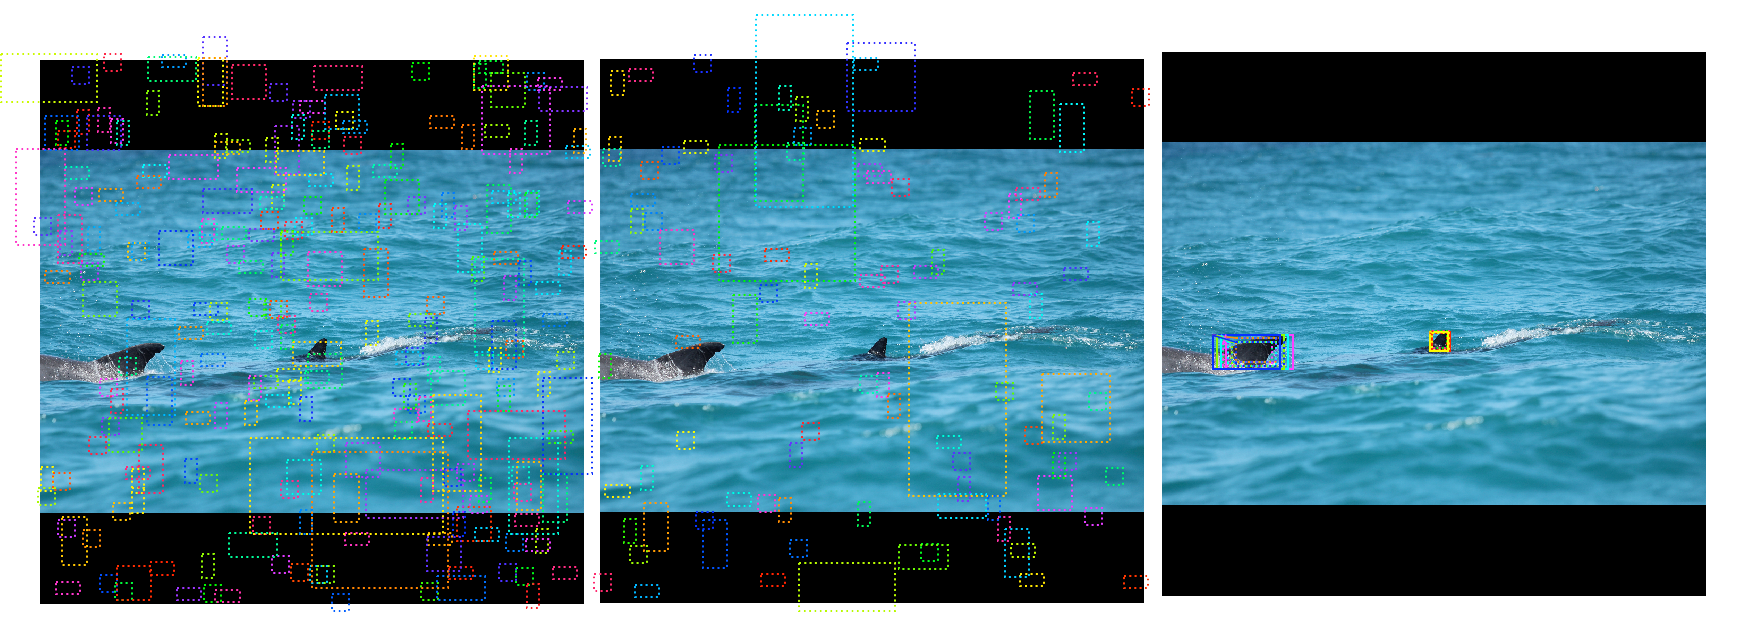
\includegraphics[scale=0.25]{Chapter2/figs/anchor-types.png}
	\end{center}
	\caption[Generated anchors.]{Generated anchors. Left: negative anchors. Middle: neutral anchors. Right: positive anchors.}
	\label{fig:anchor-types}
\end{figure}

In some cases, positive anchors may not fully cover the ground truth object. Because of this, the RPN regresses a refinement applied to the anchors, shifting and resizing them to correct their encasement of the ground truth object. An example of this can be seen in Figure \ref{fig:rpn-refined}.

\begin{figure}
	\begin{center}
		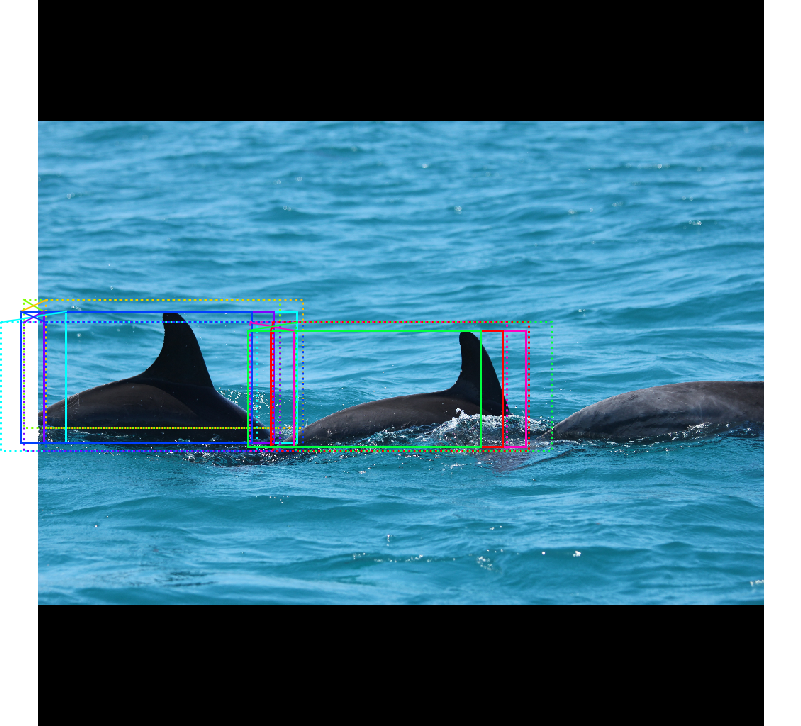
\includegraphics[scale=0.3]{Chapter2/figs/rpn-refined.png}
	\end{center}
	\caption[An example of refined anchors.]{An example of refined anchors. Positive anchors before refinement are dotted, after refinement are solid.}
	\label{fig:rpn-refined}
\end{figure}

Utilising RPNs does have disadvantages however. Generating the segmentations from the regions takes a significant amount of time, and the features generated by RPNs generally do not contain enough feature information to generate well defined masks. Recent research has attempted to fix these issues, such as SDS \cite{hariharan_simultaneous_2014} or Mask R-CNN \cite{he_mask_2017}. Work undertaken in this thesis makes use of Mask R-CNN, see Section \ref{ch:cetDet,sec:deciding} for discussion of the reasoning behind this.

Fully Convolutional Networks (FCNs)\nomenclature[z-FCN]{FCN}{Fully Convolutional Network} can also be utilised for semantic segmentation \cite{long_fully_2014}. An FCN learns pixel to pixel mappings without the need for region proposals and are built using only convolutional and pooling layers, allowing for an input image of arbitrary size (compared to classical CNNs which are generally constrained by a preset image size). This does lead to the disadvantage of down sampling the resolution of the outputted feature maps however, which sometimes causes ill-defined segmented boundaries. This issue has been tackled through the development of more advanced network architectures such as SegNet \cite{badrinarayanan_segnet:_2015}, DeepLab \cite{chen_semantic_2014, chen_deeplab_2018}, ConvNeXt \cite{liu_convnet_2022}, and PSPNet \cite{zhao_pyramid_2017}. More recent approaches to the task of semantic segmentation also make use of Transformer \cite{vaswani_attention_2017} architectures, such as Segment Anything \cite{kirillov_segment_2023} or Swin \cite{liu_swin_2021}.

Semantic segmentation can be aided through forms of supervised learning. Providing training images which have been given pixel by pixel segmentation masks can greatly improve segmentation class accuracy. Creating these masks can be extremely time consuming for researchers, and is often farmed out to external companies such as Amazon's Mechanical Turk \cite{buhrmester_amazons_2011}. However, doing this can lead to a wide variance in the quality of ground truth masks generated due to the financial incentive for those creating the masks to work as quickly as possible, necessitating the need to develop bespoke systems for quality control \cite{maji_large_2011}.

\subsection{Part Segmentation}\label{ch:Background,sec:Fine-grainedCV,sub:PartSegmentation}

In part segmentation, a coarse-grained classification is broken down into sub-components which are then analysed to provide a fine-grained identification \cite{zhang_part-based_2014}. This is still an active area of research, with some approaches focusing on a form of hierarchical part matching \cite{xie_hierarchical_2013}, some on alignment of objects to define a super-class shape \cite{gavves_fine-grained_2013}, some utilising deformable part descriptors \cite{zhang_deformable_2013}, and others using part localisation \cite{liu_dog_2012}.

At first glance it may seem as though part segmentation would be useful for this thesis' work into automatic photo-id. However, when analysing the target data it becomes apparent there would be little benefit to this approach over other segmentation techniques. As this work focusses on above water photo-id the vast majority of images observed by the developed system only contain one part of the animal -- the dorsal fin as it breaches the waterline.  As such there would be little advantage to the use of part segmentation here, as only one part is visible. If this work shifted focus to include underwater photo-id, part segmentation would be extremely useful. In this case there would be multiple parts of the animal visible such as the dorsal, tail stock, head, ventral, or sides. Each of these parts would have their own prominent markings useful for identification. However even if all parts of the animal are visible, it may be the case due to water conditions that not all prominent markings are. Algal bloom and light refraction can obscure an individual's identifying information, and so it would be very useful to be able to break down an individual using part segmentation, allowing for identification to be performed on each part rather than the whole animal, potentially increasing the chance of identification.  

\subsection{Instance Segmentation}\label{ch:Background,sec:instanceSegmentation}

Building on the concept of semantic segmentation, instance segmentation can be performed when further detail about an image is required by a developed system. Whilst many of the underlying processes are similar between the two segmentation types, instance segmentation allows for the model to distinguish between multiple objects which are of the same class; an example of this can be seen in Figure \ref{fig:masks-example}.

\begin{figure}
	\begin{center}
		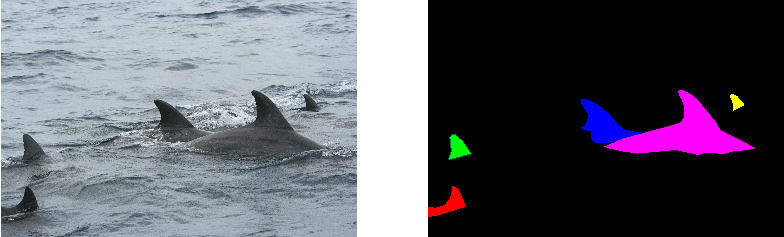
\includegraphics[scale=0.5]{Chapter2/figs/masks-example-updated-colours.png}
	\end{center}
	\caption[Left: an example of some input image. Right: the corresponding \texttt{dolphin} ground truth instance segmentation masks.]{Left: an example of some input image. Right: the corresponding \texttt{dolphin} ground truth instance segmentation masks. Each mask is highlighted a different colour, with background denoted black.}
	\label{fig:masks-example}
\end{figure}

As such, instance segmentation provides a far more detailed explanation of the input image. This information can be invaluable if the developed system is required not only to understand what pixel classes are present in the input image, but also how many of these class instances there are. These systems are often expensive to develop, however, due to the increased workload of data labelling required. Compared to data labelled for object detection, which only requires a bounding box ground truth, instance segmented data is required to be labelled on a pixel basis in a similar manner as semantically segmented data. However instance segmented data requires each pixel be assigned a specific object if there are multiple objects of the same class in the image which is not the case for semantically segmented data.

In a sense, instance segmentation can be seen as combining both object detection and semantic segmentation into one task. Traditionally, however, in order to achieve the goal of instance segmentation, proposed systems have kept the two tasks divided. These traditionalist methods take one of two approaches. 

The first, known as top-down, begins by detecting objects of interest via an RPN to create bounding boxes. These detections are then fed to the mask predictor to determine which pixels inside of the boxes belong to either the target or background class. Examples of top-down approaches to instance segmentation include Mask R-CNN \cite{he_mask_2017}, built upon Faster R-CNN \cite{ren_faster_2015}, and HCT \cite{chen_hybrid_2019}, built upon Cascade R-CNN \cite{cai_cascade_2018}.

In contrast, bottom-up systems first segment then detect, such as SpatialEmbedding \cite{neven_instance_2019} which attempts to tackle instance segmentation through the use of a Gaussian function to produce a probability for a pixel being part of the background or foreground, and then performing object detection on the foreground pixels. The major similarity between both top-down and bottom-up approaches is that they are both sequential in nature, requiring one stage to happen before the other. As such, these systems are very hard to speed up. However two stage systems often perform the best in terms of accuracy, and thus are still extremely common backbones of systems requiring the use of instance segmentation \cite{soviany_optimizing_2018}.

In recent years research into the development of fast instance segmentation has shifted to utilising a one stage approach. These one stage systems are often able to achieve faster performance than their two stage counterparts, although often struggle to reach the same levels of segmentation accuracy \cite{soviany_optimizing_2018}. ExtremeNet \cite{zhou_bottom-up_2019} works to extract four ``extreme points'' and one ``center point'' of potential objects in the input image through the use of a keypoint estimation network, creating a coarse mask. ESE-Seg \cite{xu_explicit_2019} utilises the concept of Chebyshev polynomials to fit a radius around each object inside of the detected bounding box. Similarly, PolarMask \cite{xie_polarmask_2020} also represents masks through the use of a contour around the object, modelling this through the use of polar coordinates. FourierNet \cite{riaz_fouriernet_2020} builds on this radius concept further through the use of a Fourier transform to smooth the contour. This contouring of the object is extremely fast; however, the generated masks are very imprecise. Further, any objects which contain spaces or holes, such as doughnuts, would not be able to be accurately represented. 

YOLOACT \cite{bolya_yolact_2019} builds on the well known YOLO object detection architecture, specifically YOLOv3 \cite{redmon_yolov3_2018}, adding a branch for mask prediction, but performing this through the use of two parallel tasks. The first utilises an FCN to generate prototype masks, whilst the second predicts instance coefficients. These can be combined into one mask through matrix multiplication operations with the detected bounding box. BlendMask \cite{chen_blendmask_2020} works in a similar way to YOLOACT, however, it predicts an attention map rather than instance coefficients and utilises FCOS \cite{tian_fcos_2019} as a backbone, a completely anchor and proposal free object detection architecture resulting in reduced complexity when compared to YOLO \cite{redmon_you_2016} and SSD \cite{liu_ssd:_2016}. 

Whilst the majority of one stage approaches to instance segmentation rely on bounding boxes, this is not always the case. SOLO \cite{wang_solo_2020} introduces the concept of instance categories, assigning these to each pixel according to the size and location of the instance. SOLOv2 \cite{wang_solov2_2020} builds on SOLO through the implementation of an novel non-maximum suppression algorithm. SOLOv2 often depicts higher quality masks than more often used two-stage systems such as Mask R-CNN and is able to perform real-time inference. Further, the use of Transformer \cite{vaswani_attention_2017} architectures such as Mask DINO \cite{li_mask_2022} and EVA \cite{fang_eva_2022} has allowed for state-of-the-art instance segmentation results to be obtained on a variety of benchmark datasets. It should be noted however that these architectures are recent additions to the instance segmentation arsenal, with SOLO and SOLOv2 released in 2020 whilst Mask DINO and EVA were published in 2022. 

\subsubsection{Mask R-CNN}\label{ch:Background,sec:instanceSegmentation,sub:Mask R-CNN}

As discussed in previous sections, there are multiple standardised architectures utilised for segmentation tasks. As such, when developing a system that utilises segmentation, developers of these systems will, more often than not, use one of the many architectures from the literature rather than developing their own custom architecture. Utilising one of the standard architectures has many advantages; for one, researchers do not need to spend time creating a model architecture for their task, allowing for development in other, novel areas. Further to this, utilising a standard architecture allows for research to be more easily understood and reproduced. As this thesis focusses on the automation of photo-identification systems rather than on the development of new novel architectures, it makes sense to make use of an architecture that is well known, has a track record of performing well when trained on non-benchmark or custom datasets, and is easily reproducible. As such, parts of this project's automation pipeline make use of Mask R-CNN. Because of this, it is important to understand Mask R-CNN in more detail compared to the other architectures discussed previously in this chapter. 

As seen previously, it is often the case that new architectures either extend or borrow features from older ones. This is also the case with Mask R-CNN, developed in 2017 by He \textit{et al.} \cite{he_mask_2017} on top of the existing 2016 Faster R-CNN architecture from Ren \textit{et al.} \cite{ren_faster_2015} (itself an extension of Fast R-CNN developed in 2015 \cite{girshick_fast_2015}). 

Faster R-CNN is a two stage architecture. The first stage utilises a standard backbone network such as ResNet \cite{he_deep_2015}, VGG \cite{simonyan_very_2015}, or Inception \cite{szegedy_going_2015}, to convert an input image into a set of feature maps which are passed to an RPN for analysis (see Section \ref{ch:Background,sec:objectDetection,sub:RPN} for a breakdown of RPNs). This RPN generates region proposals which are passed to the second stage of Faster R-CNN, along with the previously generated feature maps, and fed to an RoI pooling layer.  Here, each proposed region and corresponding feature map is utilised to predict bounding boxes, classifications, and confidence scores. A visual representation of Faster R-CNN's architecture can be seen in Figure \ref{fig:faster-r-cnn-architecture}.


\begin{figure}
	\begin{center}
		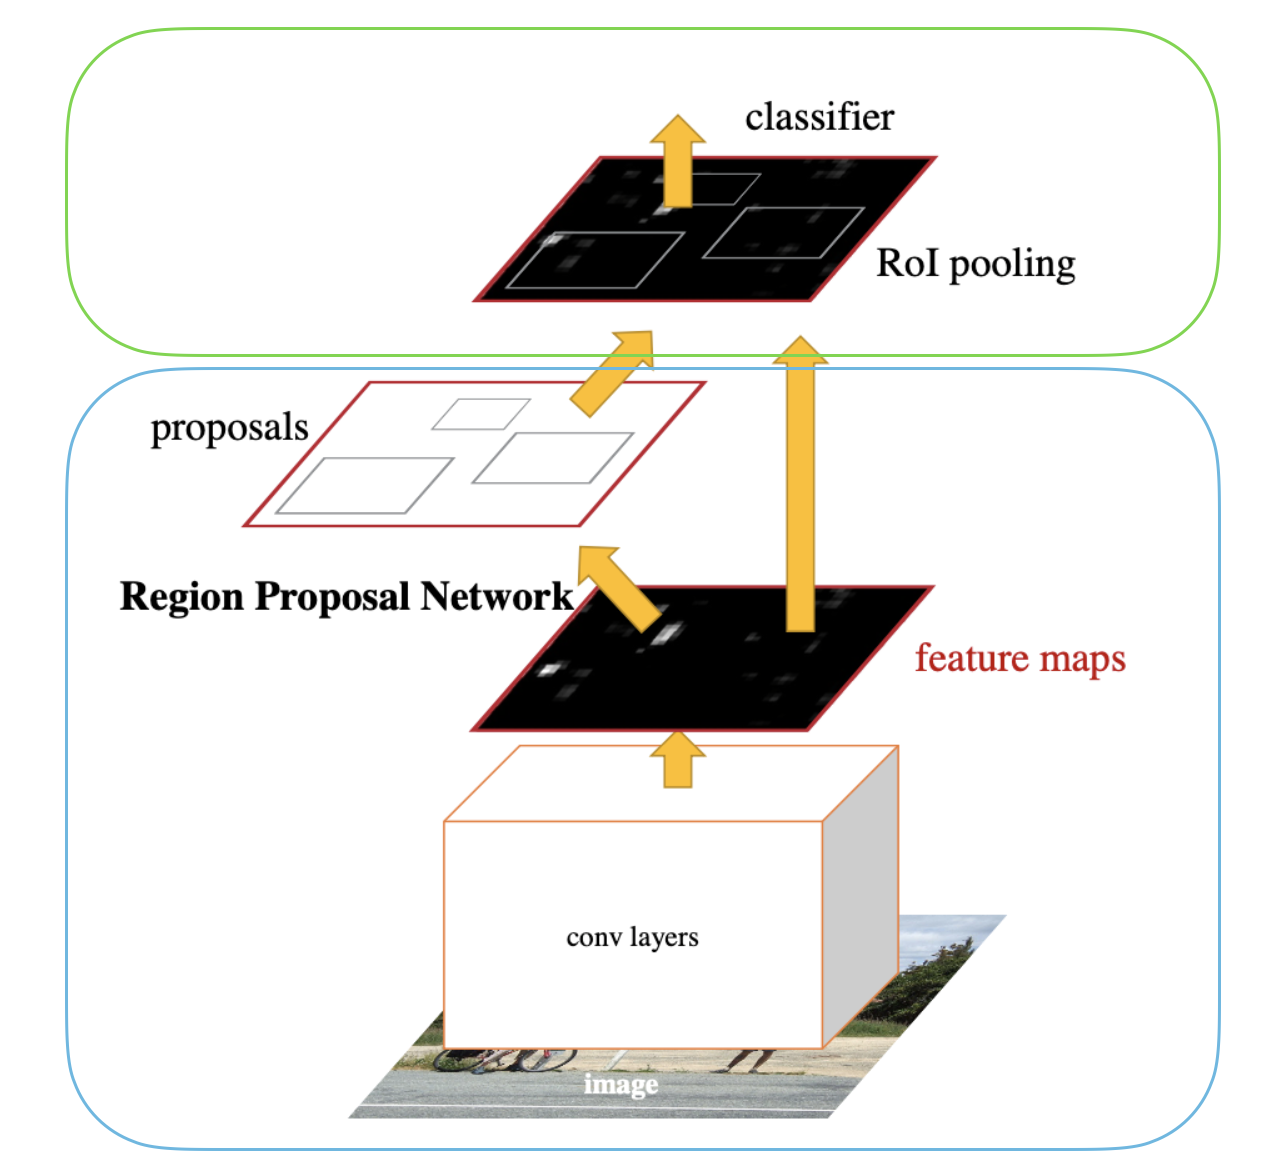
\includegraphics[scale=0.5]{Chapter2/figs/faster-r-cnn-architecture.png}
	\end{center}
	\caption[The Faster R-CNN architecture.]{The Faster R-CNN architecture \cite{ren_faster_2015}. The blue box represents operations in stage one, which includes a standard backbone CNN architecture and RPN. The green box represents operations in stage two, performing RoI pooling and classification.}
	\label{fig:faster-r-cnn-architecture}
\end{figure}

Mask R-CNN extends Faster R-CNN, allowing for instance segmentation through some relatively simple changes and additions to stage two of the architecture. First, the RoI pooling layer is replaced with an RoI align layer. This replacement layer removes the ``harsh quantisation'' which is present in RoI pooling, and properly aligns the extracted features with the input image. Second, an additional branch is added to the end of stage two. This branch receives the output of the new RoI align layer and processes it using a mask head, consisting of additional convolutional layers which generate pixel predictions and instance mask outputs. See Figure \ref{fig:mask-r-cnn-changes} for a visual representation of the changes made by Mask R-CNN.  

\begin{figure}
	\begin{center}
		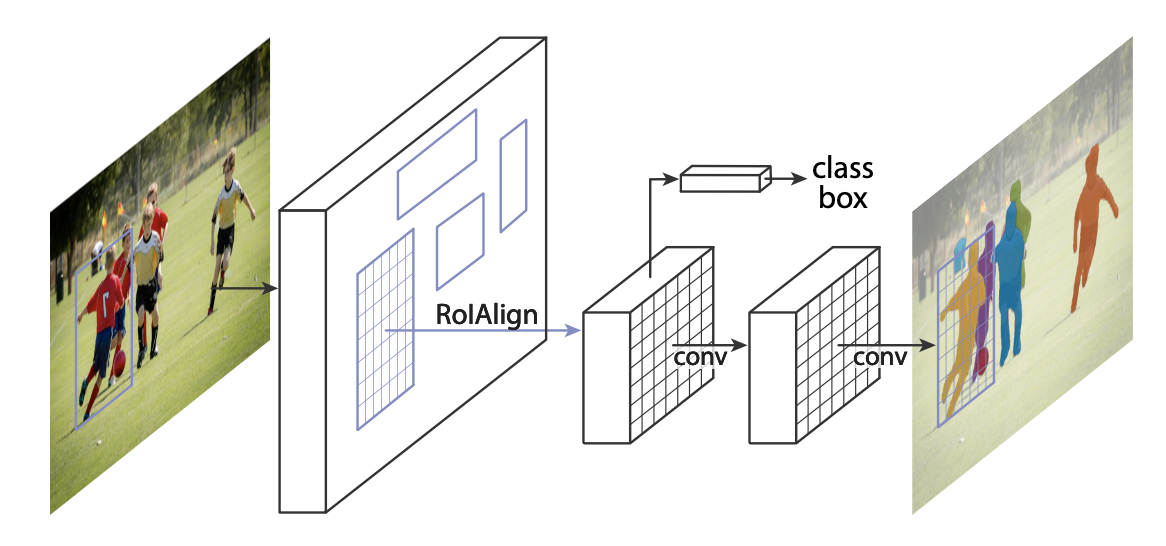
\includegraphics[scale=0.5]{Chapter2/figs/mask-r-cnn-changes.png}
	\end{center}
	\caption[A visual representation of the changes made to stage two of Faster R-CNN to create Mask R-CNN.]{A visual representation of the changes made to stage two of Faster R-CNN to create Mask R-CNN. The RoI Pooling layer has been replaced with an RoI Align layer, along with the addition of a mask head. Image from \cite{he_mask_2017}.}
	\label{fig:mask-r-cnn-changes}
\end{figure}

Thanks to these additions, Mask R-CNN is able to perform extremely accurate instance segmentation with a relatively small drop in inference speed, even when predicting on custom datasets. This speed is greatly valuable when a large number of images are required to be processed in a batch manner, such as overnight in between photo-id surveys. Indeed the use of Mask R-CNN for instance segmentation in the literature is far ranging, being utilised in medical \cite{rohit_malhotra_autonomous_2018, chiao_detection_2019, liu_segmentation_2018, anantharaman_utilizing_2018}, agricultural \cite{qiao_cattle_2019, zhao_comparing_2018, lee_potato_2020, chu_deepapple_2020}, sports \cite{buric_ball_2018, pobar_detection_2019, nguyen_hand_2018}, astronomical \cite{burke_deblending_2019}, and nautical \cite{nie_inshore_2018, hong_trashcan_2020} fields. Alongside being well known, Mask R-CNN is also extremely reproducible. An official PyTorch implementation is available \cite{wu_detectron2_2020}, though Matterport's implementation is most commonly utilised when working with Tensorflow (including in this thesis) \cite{waleed_mask_2017}.

\subsection{Fine-Grained Visual Categorisation}\label{ch:Background,sec:Fine-grainedCV}

Categorisation of objects through the use of machine learning may at first glance look like a solved problem. Indeed, it is now possible to achieve better than human levels of accuracy on a wide variety of tasks; at the time of writing the current state of the art for ImageNet \cite{deng_imagenet:_2009} and CIFAR-10 \cite{krizhevsky_learning_2009}, two of the most commonly used classification benchmark datasets, are both held by Foret \textit{et al.} \cite{foret_sharpness-aware_2020} utilising EfficinetNet with SAM at 88.61\% and 99.70\% top-1 accuracy respectively. However, it is important to note that all of these tasks are coarse-grained in nature. Benchmark datasets usually contain classes which are relatively distinct, for example \texttt{cat}, \texttt{dog}, and \texttt{ship} classes in CIFAR-10, which all have large inter-class variation. 

In contrast to the coarse-grained nature of the datasets above, fine-grained datasets are those with a small inter-class variation. Whilst CIFAR-10 has one class covering all different types of \texttt{dog}, the fine-grained dataset Stanford Dogs \cite{khosla_novel_2011} is made up of 120 classes each containing examples of only one dog breed (\texttt{chihuahua}, \texttt{beagle}, etc.). Other common fine-grained benchmark datasets often focus on wildlife or vehicles, including Caltech-UCSD Birds 200 \cite{welinder_caltech-ucsd_2010}, the updated Caltech-UCSD Birds 200-2011 \cite{wah_caltech-ucsd_2011}, and FGVC Aircraft \cite{maji_fine-grained_2013}. 

Whilst fine-grained datasets may contain small inter-class variation, their intra-class variation can be relatively large (although not larger than the inter-class variation). Class examples may contain a wide variety of orientations, poses, colour, and sizes. This allows for trained models to generalise and be capable of detecting class examples in a wider variety of cases. It is also important to note here that models which perform well on coarse-grained data are not guaranteed to do so on fine-grained data. For example EfficientNet with SAM which, as previously stated, is state of the art in multiple coarse-grained tasks however ranks 31\textsuperscript{st} in the FGVC Aircraft benchmark ranking on Papers With Code\footnote{Papers With Code -- FGVC Aircraft Rankings: \href{https://paperswithcode.com/sota/fine-grained-image-classification-on-fgvc}{paperswithcode.com/sota/fine-grained-image-classification-on-fgvc}} at the time of writing.

\subsection{Extreme Fine-Grained Visual Categorisation}\label{ch:Background,sec:ExtremeFine-grainedCV}

Residing at the end of the scale of classification granularity is the task of extreme fine-grained classification, where the differences between dataset classes are minute. Developing extreme fine-grained datasets is extremely difficult, often requiring the input of domain experts to label class examples. Taking photo-id data as an example, at a coarse-grained level it would be enough to label all classes in a photo-id catalogue as \texttt{dolphin}. At a fine-grained level multiple classes may start to exist, such as splitting based on species. Building a useable photo-id catalogue however is an extreme fine-grained task, where classes are split based on the individual. 

Often there will be very few prominent markings which will allow for an individual to be classified, and these markings are often very small such as a notch in the fin or a scar; the vast majority of pixels in the classes will be very similar. Because of this, photo-id catalogues can only be accurately produced by local marine ecologists who have studied the resident cetacean population for many years. Even with this expertise however, creating an extreme fine-grained dataset such as a photo-id catalogue can be a large undertaking, often requiring many months of work to ensure all classifications are correct. An example highlighting the differences between coarse, fine, and extreme fine-grained recognition can be seen in Figure \ref{fig:granularity-differences}.

\begin{figure}
	\begin{center}
		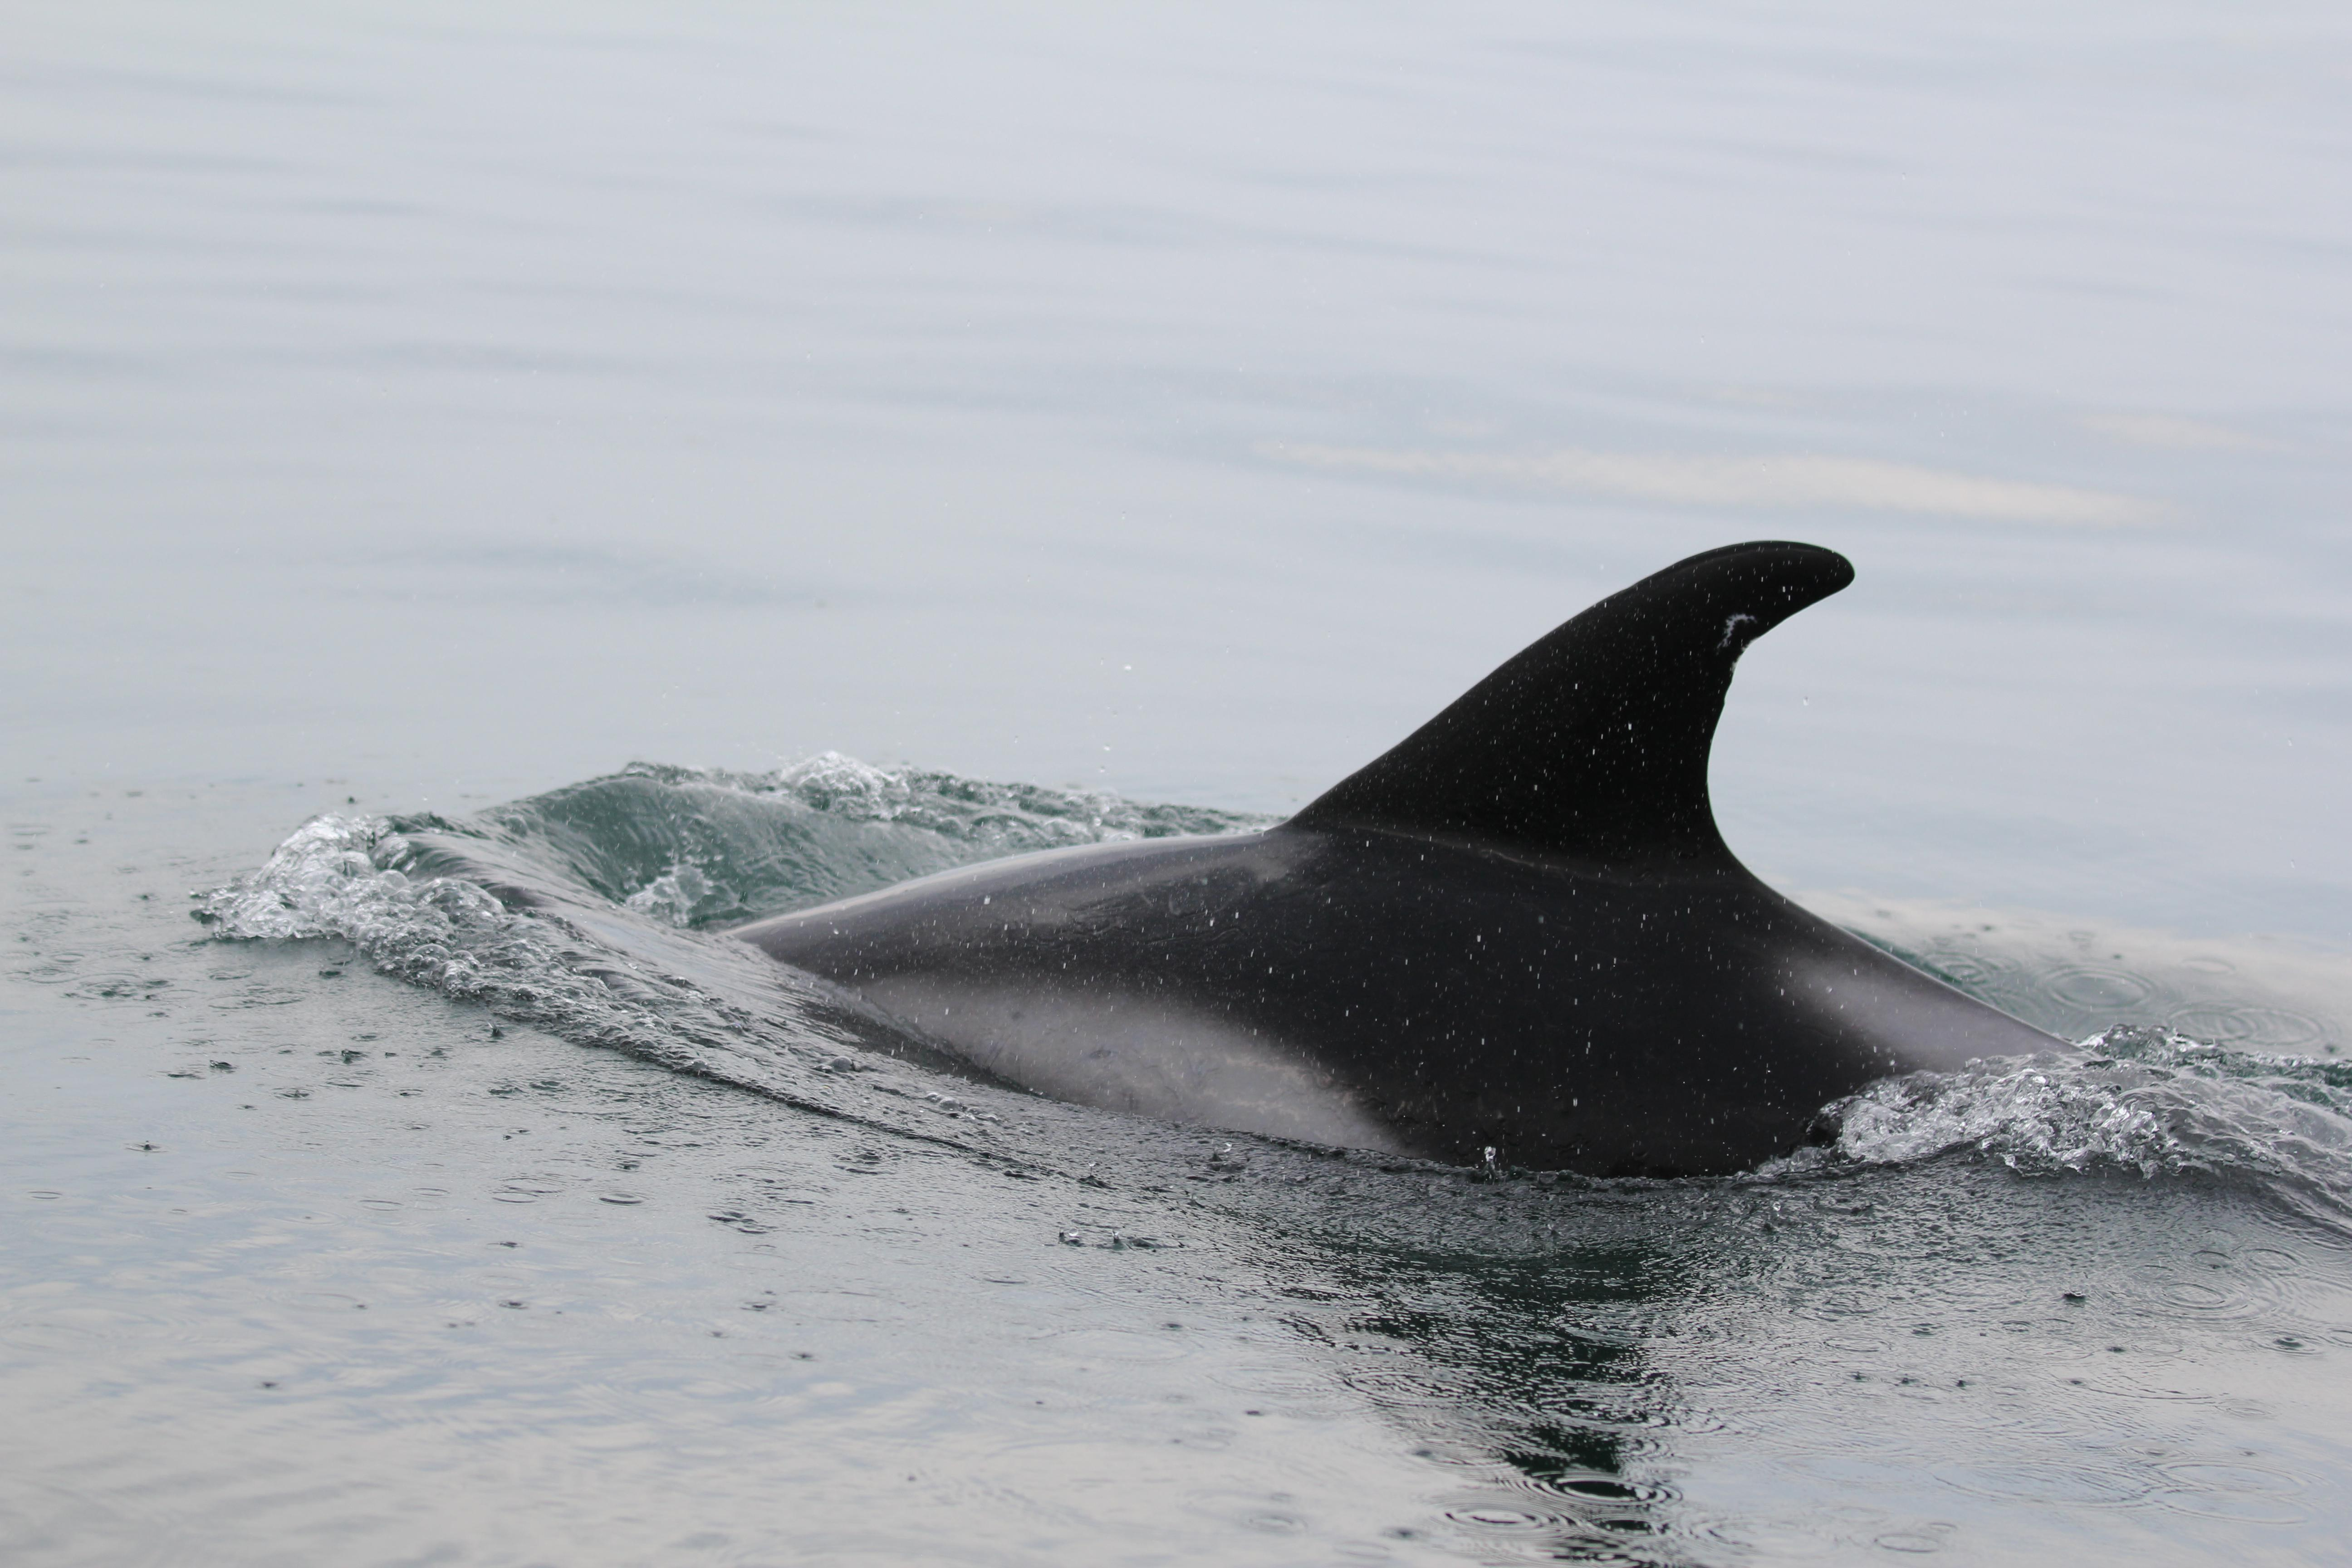
\includegraphics[scale=0.05]{Chapter2/figs/2192.jpg}
	\end{center}
	\caption[An example image from a photo-id catalogue with one individual present.]{An example image from a photo-id catalogue with one individual present. At a coarse-grained level, this individual is classed as \texttt{dolphin}, at a fine-grained level \texttt{WBD} (white-beaked dolphin), and at an extreme fine-grained level \texttt{32}, the individual's catalogue ID. Image and class labels from \cite{trotter_ndd20_2020}.}
	\label{fig:granularity-differences}
\end{figure}

\section{Computer Vision for Ecology}\label{ch:Background,sec:conTech}

Thanks to the large advances in computer vision and deep learning, and the increasing prevalence of these systems in areas such as manufacturing and healthcare, researchers have, in recent years, begun exploring other areas of society which could benefit from AI systems. One of the more niche, but arguably highly important areas where computer vision can make an impact, is ecology \cite{weinstein_computer_2018}.

Work into applying object detection and segmentation to ecology data mostly focusses on camera trap systems due to the large amount of data readily available. For example, the Snapshot Serengeti project, developed by Swanson \textit{et al.} \cite{swanson_snapshot_2015} has utilised camera traps in Tanzania's Serengeti National Park to develop a fully labelled camera trap image dataset capable of training machine learning systems. The camera traps used have been in continuous operation since 2010 and cover an area of 1125km\textsuperscript{2}. The iWildcam dataset provides further camera trap training data from across the South-western United States \cite{beery_iwildcam_2019}.

Camera traps capture a photo every time movement in the frame is detected, and as such a large proportion of the images a camera trap captures either do not contain any animals at all (e.g. wind has caused the surrounding vegetation to move), or contain animals which are not the primary species of investigation. This provides a key driver for the development of machine learning camera trap systems which could, for example, filter out erroneous captures automatically. Whilst these images may simply be discarded by the researchers, they have a use in the development of machine learning camera trap based systems, allowing them to be trained on a wide variety of examples. As such, machine learning systems developed for camera traps have found quick adoption in the research community with many systems now capable of performing fine-grained species classification with extremely high accuracy \cite{tabak_machine_2019, norouzzadeh_automatically_2018, willi_identifying_2019, beery_efficient_2019, norouzzadeh_deep_2019}. Recent work by Clapham \textit{et al.} \cite{clapham_automated_2020} has moved further to the extreme of fine-grained classification with BearID, a project which adapts human facial recognition systems for use with brown bears (\textit{Ursus arctos}) via metric embeddings, achieving an ``individual classification accuracy'' of 83.9\%. Here, BearID is not classifying the species \textit{Ursus arctos} but rather individuals within the survey area, a significant achievement given the challenge of identifying individuals within a species which lack unique markings.

As camera traps work through movement, taking a burst of images whenever the environment they observe changes -- be this due to an animal walking through the scene or wind moving foliage -- they must be kept stationary, usually mounted to grounded objects such as trees. These requirements make camera traps unsuitable for above-water marine environments, as the trap could not be attached to a stationary object at sea. Should it be possible to provide a stationary mount for the camera trap, the environment would still be unsuitable due to the rapid changing of the observed scene, due to factors such as waves, causing the camera to constantly produce image bursts. As a result, applying computer vision to marine environments is a greater challenge than on-land camera traps. This is also in part due to the relative lack of available data to train systems. Marine datasets such as FathomNet \cite{katija_fathomnet_2022} are available, although its focus is on underwater detection and classification.

Marine ecologists traditionally rely on identification from photographs taken either from the coastline, a vessel at sea, an aircraft, or Unmanned Aerial Vehicle (UAV)\nomenclature[z-UAV]{UAV}{Unmanned Aerial Vehicle}. As this requires a human operator, the size of datasets available is relatively small. Furthermore, given the high cost of data collection, marine ecology groups often keep a tight grip on their data. This has led to a lack of available open-source datasets for those who wish to train machine learning systems for use in marine ecology. Thanks to advances in UAV technology and their current inexpensiveness, some research groups have shifted focus to the use of UAVs for image capture. This new approach has seen success in areas such as photo-identification \cite{bogucki_applying_2019, gray_drones_2019}, microbial sampling \cite{centelleghe_use_2020}, and human-interaction response monitoring \cite{fiori_using_2020}. However, some recently published work highlights the need to better understand how UAVs affect the behaviour and health of marine species \cite{giles_responses_2020, bevan_measuring_2018, ramos_bottlenose_2018, pomeroy_assessing_2015}. 

\subsection{Utilising Photo-id Aids in Cetacean Research}\label{ch:Background,sec:conTech,sub:photoIDAides}

Performing manual analysis of photo-id surveys with the goal of creating a catalogue can be extremely time consuming and labour intensive. Images collected during fieldwork are brought back to the lab and filtered, removing images which do not contain cetaceans. The remaining images are then often pre-processed through a combination of manual orientation shifts and crops to centre and isolate the dorsal fin -- any with more than one fin are split into multiple images at this stage. Next, the fins present in the images are identified by multiple researchers, either using an existing catalogue to compare against or building this using the data if one does not currently exist. These researchers are often experts in their field, having performed photo-id catalogue matching for many years, with multiple experts utilised to reduce the risk of misidentifications. 

Due to the lengthy and expensive nature of manual photo-id, multiple aids have been developed over the years to ease the process. These have advanced at pace, gradually reducing the amount of human interaction and manual pre-processing of the data seen by these systems. A description of existing programs and academic literature is now provided, with an overview in Table \ref{tab:Photo-IDAidesComparison}.

\begin{table}
	\caption[A comparison of available photo-id aids.]{A comparison of available photo-id aids.}\label{tab:Photo-IDAidesComparison}
	\begin{adjustbox}{width=\columnwidth, center}
		\begin{tabular}{*{8}{c}}
			\toprule
			System                 &     \begin{tabular}[c]{@{}c@{}}Catalogue Size\\(If Known)\end{tabular}                                                                             & \begin{tabular}[c]{@{}c@{}}Requires\\Data Pre-processing\end{tabular} & \begin{tabular}[c]{@{}c@{}}Dorsal Fin\\Detection\end{tabular}             & \begin{tabular}[c]{@{}c@{}}Full\\ Background Removal\end{tabular} & \begin{tabular}[c]{@{}c@{}}Individual\\Photo-ID\end{tabular}                         & \begin{tabular}[c]{@{}c@{}}Can Flag Individuals\\Not Currently In Catalogue\end{tabular} & \begin{tabular}[c]{@{}c@{}}Uses All Information\\Found on Dorsal\end{tabular} \\ \hline
			FinScan \cite{hillman_finscan_2002}    & 190                                                       & \cmark                                                           & \xmark & \xmark                                             & \cmark            & \cmark                                                & \textthreequartersemdash                                  \\
			FinBase \cite{adams_automating_2006}     & 409                                                     & \cmark                                                           & \xmark & \xmark                                             & \cmark            & \cmark                                                & \textthreequartersemdash                                  \\
			DARWIN \cite{hale_unsupervised_2012}  & 200                                                         & \cmark                                                           & \xmark & \xmark                                             & \cmark            & \cmark                                                & \textthreequartersemdash                                  \\
			catRlog \cite{keen_catrlog_2021}   & \textthreequartersemdash                                                            & \cmark                                                           & \xmark & \xmark                                             & \cmark            & \cmark                                                & \textthreequartersemdash                                  \\
			CurvRank \cite{weideman_integral_2017}  & 3973                                                     & \cmark$^*$                                                           & \xmark$^*$ & \xmark                                             & \cmark            & ?                                                                    & \xmark                                  \\
			Karnowski \textit{et al.} \cite{karnowski_dolphin_2015}    & \textthreequartersemdash                   & \xmark                                                           & \cmark & \cmark                                             & \xmark            & \textthreequartersemdash                              & \textthreequartersemdash                                  \\
			Photo-ID Ninja\textsuperscript{\ref{footnote:photo-idNinja}}  & \textthreequartersemdash                  & \xmark                                                           & \cmark & \xmark                                             & \xmark            & \textthreequartersemdash                              & \textthreequartersemdash                                  \\
			Qui\~{n}onez \textit{et al.} \cite{quinonez_using_2019} & \textthreequartersemdash & \xmark                                                           & \cmark & \xmark                                             & \xmark            & \textthreequartersemdash                              & \textthreequartersemdash                                  \\
			Morteo \textit{et al.} \cite{morteo_phenotypic_2017}    & 533                      & \cmark                                                           & \xmark & \xmark                                             & \cmark            & \xmark                                                & \xmark                                                    \\
			Bouma \textit{et al.} \cite{bouma_individual_2018}  & 185                          & \cmark                                                 & \cmark$^\dagger$ & \xmark                                             & \cmark            & \cmark                                                & \cmark                                                    \\
			Lee \textit{et al} \cite{lee_backbone_2020}   & 25                                & \xmark                                                           & \cmark & \cmark                                             & \cmark$^\ddagger$ & ?                                                                    & \textthreequartersemdash                                  \\
			finFindR \cite{thompson_finfindr_2022}    & 271/149$^\divideontimes$                                                     & \xmark                                                           & \cmark & \xmark                                             & \cmark            & \cmark$^\parallel$                                               & \xmark                                                    \\
			\begin{tabular}[c]{@{}c@{}} Georgetown University \\\& Google \cite{georgetown_university_is_2018} \end{tabular}& $>$1800$^\nabla$  & \cmark & \xmark & \xmark & \cmark & \xmark & \xmark \\
			DolFin \cite{maglietta_dolfin_2018}   & 60                                          & \xmark                                                           & \cmark & \cmark                                             & \cmark$^\mathsection$            & \cmark                                                & \cmark                                                    \\ \hline
			Ours          & 43/23$^\flat$                                                                                                  & \xmark                                                           & \cmark & \cmark                                             & \cmark            & \cmark                                                & \cmark                                                    \\
			\bottomrule
		\end{tabular}
	\end{adjustbox}
	{\raggedright\footnotesize{* Flukebook\textsuperscript{\ref{footnote:flukeBook}} can perform automatic data pre-processing and fin detection before passing the output to CurvRank, but the algorithm itself does not facilitate this. \\ ? It is unclear whether the system is capable of flagging previously uncatalogued individuals. \\ $\dagger$ Utilises Photo-ID Ninja\textsuperscript{\ref{footnote:photo-idNinja}} for detection. \\$\ddagger$ Sparse on detail regarding photo-id performance.\\$\divideontimes$ Evaluation utilises ``full'' (n = 271) and ``reduced'' (n = 149) datasets. \\$^\parallel$ Individuals not present within the top-50 most likely are considered be previously uncatalogued.\\$\nabla$ Exact number not given. \\$\mathsection$ Utilises SURF for photo-id, thus unsuitable for cetacean species without well-defined markings. \\ $\flat $ Most likely catalogue matching evaluated using the NDD AU SMRU (n = 43 plus \texttt{noise}), see Section \ref{ch:ID,sec:ModelSelection}, and the SDRP datasets (n = 23), see Section \ref{ch:SNNEvaluation,sec:SDRP}.}}
\end{table}

\subsubsection{Catalogue Management Systems}\label{ch:Background,sec:conTech,sub:photoIDAides,subsub:databases}

Due to the potential size of photo-id catalogues, especially in geographic locations with large populations, many aids focus on the management of these catalogues using databases. The first of these, FinScan, was developed in 2000 \cite{hillman_finscan_2002}. This is a semi-automated photo-id assistant whereby the user imports images taken during fieldwork. FinScan then attempts to create a trace of the fin in the image. Users may manually edit this trace however if it is not exact (this feature was developed due to frustration with barnacles attaching to fins in the area where FinScan was developed). The trace of the fin is then checked against a local Microsoft Access database to determine close matches which are presented to the user. Before images are imported into FinScan they must be manually cropped, sharpened, and rotated by the user. Rotation of the image is especially important, as the FinScan algorithm is not rotation invariant. Whilst FinScan is freeware it is no longer readily available. Anyone who wishes to use it must procure a copy from someone else, there is no central repository for downloading. Issues with running the software on newer systems may also be present.

Similarly to FinScan, FinBase is a photo-id database management system developed by NOAA Fisheries \cite{adams_automating_2006}. However, unlike other systems, FinBase provides no matching based on automatically generated fin properties; instead, FinBase facilitates matching through user defined attributes. These could be physical descriptors such as `top notch' or `skin disorder' but may also be non-physical attributes if the user wishes. Fins are partially matched based on querying the backend database for entries which also have the attributes of those inputted by the user for the query fin. 

{
	\stepcounter{footnote}\footnotetext{\label{footnote:photo-idNinja}Photo-ID Ninja: \href{http://photoid.ninja}{photoid.ninja}}
	\stepcounter{footnote}\footnotetext{\label{footnote:flukeBook}FlukeBook: \href{https://www.flukebook.org/}{flukebook.org}}
}

Alongside both of these, DARWIN \cite{hale_unsupervised_2012} provides automated identification of new images based on those already in the attached database. Like FinScan, users of DARWIN trace around the leading and trailing edges of the fin they wish to identify. These edges are stored in a database as a set of evenly spaced points approximating the outline of the fin which is then used for identification.

CatRlog \cite{keen_catrlog_2021} is an R Shiny based catalogue management system which allows for photo-identification of individual cetaceans. Researchers enter descriptions manually for unique markings located on either the dorsal fin or fluke of the individual. One of catRlog's main advantages is the ability to be hosted locally on machines via RStudio whilst also being capable of handling catalogues hosted on cloud-based storage solutions. This allows for efficient id verification, as multiple experts can id images at the same time each uploading results to the central catalogue. If any discrepancies arise, such as an individual given a different id by multiple experts, this centralised approach allows for the catalogue manager to easily determine the final id and disseminate this to other catalogue users. CatRlog is also capable of automated print-friendly photo-id catalogue creation. 

\subsubsection{Classical Machine Learning Systems}\label{ch:Background,sec:conTech,sub:photoIDAides,subsub:nonDL}

Multiple systems which utilise classical machine learning are also available to aid cetacean researchers. Karnowski \textit{et al.} \cite{karnowski_dolphin_2015} propose using Robust Principal Component Analysis (PCA)\nomenclature[z-PCA]{PCA}{Principal Component Analysis} to subtract background from underwater images to help detect captive bottlenose dolphins and track their movements through multiple distinct areas. CurvRank is an algorithm developed by Weideman \textit{et al.} \cite{weideman_integral_2017} which automatically identifies the trailing edge of the fin and represents this as a set of ordered coordinates. Each coordinate point then has a circle of radius $r$ placed upon it, before being transformed horizontally. The curvature at this point for a given $r$ value is then defined as the ratio of the area under the curve against the area of a square around the curve of length $2r$. This allows for the definition of the trailing edge of the fin to be rotation invariant. Whilst initially developed for cetaceans, CurvRank has also found use in land-based photo-id surveys due to its robustness. For example, Kulits \textit{et al}. \cite{kulits_elephantbook_2021} utilise CurvRank and SEEK \cite{bedetti_system_2020} as the basis for a human-in-the-loop system for African elephant (\textit{Loxodonta africana}) photo-id. 

\subsubsection{Deep Learning Systems}\label{ch:Background,sec:conTech,sub:photoIDAides,subsub:DL}

In recent years the use of deep learning has been explored, inching forward towards a fully automatic photo-id system. One of the main labour costs in the creation of photo-id catalogues is the processing of survey data. This is usually cropping the images collected down to just the fins in the image, removing unneeded background. Photo-ID Ninja\textsuperscript{\ref{footnote:photo-idNinja}} is designed to speed up this processing. Users provide a batch of images taken directly from the field to the system, which utilises an object detection model to output bounding boxed dorsal fins which can then be manually identified.

Qui\~{n}onez \textit{et al.} \cite{quinonez_using_2019} propose a CNN based system capable of cetacean object detection, detecting four distinct classes: \texttt{dolphin}, \texttt{dolphin\_pod}, \texttt{open\_sea}, and \texttt{seabirds}. Morteo \textit{et al.} \cite{morteo_phenotypic_2017} perform semi-automatic fin measuring using fin shape in order to aid in population monitoring. This technique, based on work by Weller \cite{weller_global_1998}, does not require the user to trace the fin; instead lines are projected out from the base of the leading edge of the fin, with the user cutting these lines where they intersect with a point on the trailing edge. 

Bouma \textit{et al.} \cite{bouma_individual_2018} provide a system focusing on learned metric embeddings in order to photo-id individual New Zealand common dolphins (\textit{Delphinus spp}). This research utilises Photo-ID Ninja to detect and crop fins before they are passed for identification, focussing on common dolphins as data subjects. The system is capable of achieving top-5 accuracy scores of around 93\%, although it should be noted here that the data utilised to achieve this score is not currently publicly available. An attempt to obtain this data was undertaken, but no response was received. As such, it is not possible to determine how distinct each individual is in the dataset. Based on the figures presented in the paper, it seems no segmentation of the cropped fins is performed before they are embedded. As such, some noise in the embeddings will be present. 

FinFindR is an algorithm developed by Thompson \textit{et al.} \cite{thompson_finfindr_2022} which allows for inputted images containing bottlenose dolphins to be identified. FinFindR works with un-cropped images, automatically cropping any dolphin present using a neural network. Cropping can be performed on either the whole body or on the dorsal fin only. Cropped dorsal fins are then passed to a second neural network which creates an embedding of the trailing edge of the fin. This embedding is mapped into a high dimensional space based on work presented in FaceNet \cite{schroff_facenet_2015}, with clustering of individuals achieved using Ward's variance minimising clustering \cite{ward_hierarchical_1963}. Reported accuracies for finFindR currently stand at a top-1 accuracy of 88\%, top-5 accuracy of 94\%, and top-50 accuracy of 97\%. It should also be noted that finFindR has currently only been tested on bottlenose dolphins and work is still ongoing.

Work undertaken by Georgetown University and Google in the area of cetacean photo-id has also provided promising results \cite{georgetown_university_is_2018}. The system, which utilises Google's Cloud Auto ML framework, can quickly identify bottlenose dolphins from Australia's Shark Bay. This system shows users the top-200 closest matches along with their confidence scores utilising both the leading and trailing edges of the fin. It is reported that this system saves Georgetown University's cetacean team around 4500 hours per year, highlighting the need for systems such as these to researchers in this field. However, this system does not link to a backend database to log matches found -- this must be done manually by the researchers. Further, any new individuals that need to be added to the system, or indeed if the system was to be redeployed to a new area, then all training of the underlying model must be performed by Google engineers rather than locally by the researchers who wish to utilise the system. Further, fins to be identified must be inputted one by one, no batch input function exists.  

Recent work undertaken by Lee \textit{et al}. \cite{lee_backbone_2020} proposes a novel architecture for cetacean identification. The proposed system is capable of detecting small objects in large images, and utilises this for fin detection. Next, segmentation is performed using U-Net \cite{ronneberger_u-net_2015}. The resultant output is then passed to a post-processor which re-aligns and normalises the fin. The most significant features of the fin are then extracted and passed to a VGG based system \cite{simonyan_very_2015} combined with a novel V2BC component for identification, although results achieved for identification in the paper are sparse.

Maglietta \textit{et al}. \cite{maglietta_dolfin_2018} propose DolFin, a Speeded-Up Robust Features (SURF)\nomenclature[z-SURF]{SURF}{Speeded-Up Robust Features} based identification system \cite{bay_speeded-up_2008} built upon in work undertaken by Renò \textit{et al.} \cite{reno_sift-based_2019} for identifying individual Risso's dolphins. As mentioned in Section \ref{ch:Background,sec:photo-id}, this species is susceptible to prominent long-term scarring, and thus is well suited to feature detection algorithms such as SURF, with published results showing a much greater identification accuracy can be achieved compared to utilising common photo-id aids such as DARWIN \cite{hale_unsupervised_2012}. DolFin also makes use of a ``fin mask extraction'' unit capable of detecting, segmenting, and post-processing fins before they are identified using SURF, although details on this unit are unclear. This system is truly fully autonomous, although due to the SURF based system would only be capable of working with Risso's dolphins. Other cetacean species do not develop as prominent scarring, which would greatly reduce the effectiveness of SURF-based feature extraction systems. 

\subsubsection{Online Tracking Systems}\label{ch:Background,sec:conTech,sub:photoIDAides,subsub:OnlineTracking}

Whilst the use of photo-id catalogues for resident populations is beneficial for researchers in the animal's local area, some cetacean species traverse large geographical distances, sometimes travelling between continents. In these cases it would not be feasible for one research group to record sightings. This is where online tracking systems play an important role. These websites started by allowing users to enter their own sighting data into an online database, allowing for tracking of individuals over large areas. In recent years however the focus has shifted to performing detection and identification online from unlabelled sighting images. This allows groups of users such as citizen scientists to contribute to the database, as no knowledge of the existing catalogue or training in photo-id is required.

HappyWhale\footnote{\label{footnote:happyWhale}HappyWhale: \href{https://happywhale.com/}{happywhale.com}} is a CNN based photo-id system focussing on humpback whales (\textit{Megaptera novaeangliae}). The underlying CNN for this system was developed through a Kaggle competition\footnote{Kaggle competition: \href{https://www.kaggle.com/c/whale-categorization-playground}{kaggle.com}} to identify patterns present on the tailstock of the humpbacks \cite{kaggle_humpback_2018}, utilising elements of ArcFace \cite{deng_arcface_2019} and DeepFace \cite{taigman_deepface_2014} to do so. Users interact with HappyWhale through their website, uploading images of the tailstocks encountered. The HappyWhale system then attempts to identify the individual before presenting back to the user. If the user provides location data, HappyWhale also keeps track of this to produce travel maps for the individuals, as humpback whales are known to travel vast distances in their lives. The success rate for HappyWhale varies greatly, from 99\% for ``good to high quality'' images to 50\% for full fins at 50x50px. HappyWhale struggles with partially obscured tail stocks however, and work is currently ongoing in this area. 

FlukeBook\textsuperscript{\ref{footnote:flukeBook}} is a fully automatic photo-id system capable of identification of multiple cetacean species. This system is part of a wider network of animal identification tools based on Wildbook, an open source software framework developed by non-profit organisation WildMe to facilitate the introduction of artificial intelligence into the ecology space \cite{berger-wolf_wildbook:_2017}. FlukeBook makes use of both CurvRank and finFindR when working with bottlenose and spotted dolphins (\textit{Stenella frontalis}). Whilst FlukeBook is capable of detecting and identifying individual cetaceans, the fact that it is hosted online with all submissions freely searchable may be a disadvantage for some cetacean researchers. Local photo-id catalogues are closely guarded due to the effort and expense required to collect the data, and as such some groups may prefer a local automated photo-id solution over one which requires them to hand over their data to a third party. 

\subsubsection{Summary of Available Photo-id Aids}\label{ch:Background,sec:conTech,sub:photoIDAides,subsub:Summary}

As can be seen in Table \ref{tab:Photo-IDAidesComparison}, there is a wide variety of photo-id aids currently available to researchers -- each fulfilling a different need depending on the researcher and how comfortable they are with automating parts of the photo-id process. If they prefer a fully manual approach to analysis but require storage solutions, FinScan and FinBase provide excellent catalogue management. DARWIN can then extend this through automating existing catalogue databases. 

Manual analysis is extremely time consuming however, leading to modern systems allowing for some automation of processing. For fast cropping, Photo-ID Ninja can be utilised, greatly reducing the sizes of images and removing unneeded background. Algorithms like CurvRank can then be utilised to aid in identification. 

Whilst all of these systems perform their intended task well, they are mostly stand-alone. This would require researchers to make their own data pipelines should they wish to host locally, such as Bouma \textit{et al}.  \cite{bouma_individual_2018} and their use of Photo-ID Ninja for detection before embedding using deep learning to provide catalogue matching. Should researchers feel comfortable with open-sourcing their catalogues and matching process, whilst also working with a supported cetacean species, then systems like HappyWhale or FlukeBook are most appropriate, requiring little data pre-processing whilst not requiring researchers to host multiple algorithms or solutions locally, reducing the need to create their own custom data pipelines. 

It is the work undertaken by the aforementioned solutions that motivates this thesis. A fully automated photo-id system must be capable of the following:

\begin{enumerate}

\item\textbf{Operating with no data pre-processing}: Researchers should not need to process data from fieldwork cameras before it can be handled by the system. 

\item\textbf{Detection}: The system must be capable of detecting dorsal fins present in input images. This allows researchers to pass the system all images taken in the field to reduce human workload and allow the system to operate on data which has not been pre-processed. The system must be capable of detecting multiple fins in the same image.

\item\textbf{Segmentation}: Once fins have been detected, it must be possible to segment them from the image. This aids the photo-id process by removing other fins, which may contain prominent markings, as well as background such as the sea, which may be feature heavy due to waves.

\item\textbf{Photo-ID}: The system must be capable of identifying individuals in a species agnostic manner.

\item\textbf{Flagging uncatalogued individuals}: The system must be capable of flagging individuals that have not yet been catalogued to the user. 

\item\textbf{Locally deployable}: It must be possible to deploy the system on local hardware, allowing researchers to keep full ownership of their catalogue.

\end{enumerate}

Of the works highlighted in Table \ref{tab:Photo-IDAidesComparison}, only DolFin \cite{maglietta_dolfin_2018} proposes a fully automated photo-id aid which can be locally run, requires no data pre-processing, and is capable of handling uncatalogued individuals. However as previously stated this solution utilises SURF \cite{bay_speeded-up_2008}. This algorithm, like its predecessor Scale-Invariant Feature Transform (SIFT)\nomenclature[z-SIFT]{SIFT}{Scale-Invariant Feature Transform} \cite{lowe_object_1999}, excels at detecting well defined features in images. This is appropriate for DolFin's data subjects, Risso's dolphins, due to the well defined scarring patterns present on their dorsal fins \cite{mariani_analysis_2016}. The algorithm would be expected to fail when used on other cetacean species however due to a lack of well defined features on the fin, where even prominent markings used for photo-id fail to be extracted. In contrast, this thesis makes use of a robust embedding generation technique through the use of a trained Siamese Neural Network (SNN), allowing for the extraction of features in a species agnostic way. See Section \ref{ch:cetDet,sec:deciding,sub:boundingBoxInvestigation,subsub:SURF} for an investigation into the use of feature extraction algorithms on bottlenose dolphin dorsal fins, as well as Sections \ref{ch:ID,sec:SNNDevelopment} and \ref{ch:SNNEvaluation,sec:SDRP} for discussion of the use of SNNs to extract identifiable features from catalogues containing different species of interest collected over a range of spatio-temporal environments. 
 
According to Tyson Moore \textit{et al.} \cite{tyson_moore_rise_2022}, finFindR is the most commonly used photo-id aid. However, this system does not perform full background removal, which may influence the matching process as seen in Section \ref{ch:SNNEvaluation,sec:EffectOfNoise}. Furthermore, individual identification is performed using the trailing edge of the dorsal fin only, rather than all available prominent markings. Alongside this, the flagging of potentially uncatalogued individuals is performed implicitly, with input images considered previously uncatalogued if a match is not obtained with any of the top-50 most likely matches -- assuming a similar data distribution to the catalogue used to evaluate system performance \cite{thompson_finfindr_2022}. This may cause issues when working with catalogues containing significantly more than 50 individuals. In contrast, the photo-id aid outlined in this thesis performs full background removal, makes use of all prominent markings, and explicitly flags potentially uncatalogued fins to the user. For a comparison between finFindR and the photo-id aid developed in this thesis, see Section \ref{ch:SNNEvaluation,sec:FinFindRComparison}.

Work by Bouma \textit{et al.} \cite{bouma_individual_2018} also makes use of embedding generation to perform most likely catalogue matching. However, this work is not stand alone, requiring users to make use of dorsal fin detectors such as Photo-ID Ninja beforehand. These detections may require manual post-processing to be utilised and retain their background, which is shown in Section \ref{ch:SNNEvaluation,sec:EffectOfNoise} to potentially cause inflated evaluation metrics. 

\section{Summary}\label{ch:Background,sec:Summary}

This chapter presents the key ideas required to understand and appreciate the novel work proposed in this thesis. An overview of deep learning and computer vision is provided, as well as an introduction to photo-id, a key methodology for mark-recapture surveys utilised by marine ecologists. A summary of previous research combining ecology and deep learning has also been provided, with a focus on marine environments and cetaceans. Before development on the system components required by an automated photo-id aid can be undertaken, datasets suitable for the training and evaluation of these components must be created. This is outlined next in Chapter \ref{ch:datasetCreation}.

%%%%%%%%%%%%%%%%%%%
